% Select document class: uncomment one of the following
\documentclass[aspectratio=169]{beamer}  % For presentation mode
%\documentclass[11pt]{article}            % For article mode
%\usepackage{beamerarticle}               % Uncomment with article class

% =============================================================================
% COMMON PREAMBLE
% =============================================================================
% =============================================================================
% Common Preamble for Network+ Lecture Series
% This file provides consistent formatting, colors, packages, and styles
% across all lecture modules for both beamer presentations and article mode
% =============================================================================

% =============================================================================
% THEME AND COLORS
% =============================================================================
\usetheme{Madrid}
\usecolortheme{whale}

% Custom colors - standardized across all lectures
\definecolor{rctcblue}{RGB}{0, 74, 136}
\definecolor{rctcgold}{RGB}{255, 199, 44}
\definecolor{networkgreen}{RGB}{0, 128, 64}
\definecolor{alertred}{RGB}{180, 0, 0}
\definecolor{aborange}{RGB}{230, 126, 34}
\definecolor{copperbrown}{RGB}{184, 115, 51}
\definecolor{faborange}{RGB}{255, 165, 0}
\definecolor{fiberyellow}{RGB}{255, 215, 0}
\definecolor{shirepurple}{RGB}{102, 51, 153}
\definecolor{ipblue}{RGB}{52, 152, 219}
\definecolor{ippurple}{RGB}{155, 89, 182}
\definecolor{vlangreen}{RGB}{39, 174, 96}
\definecolor{tcpblue}{RGB}{30, 100, 180}
\definecolor{udpgreen}{RGB}{50, 160, 80}
\definecolor{dhcppurple}{RGB}{120, 60, 160}
\definecolor{dnsyellow}{RGB}{200, 170, 50}
\definecolor{batblack}{RGB}{30, 30, 40}
\definecolor{gothamgray}{RGB}{80, 85, 95}
\definecolor{paddysgreen}{RGB}{19, 77, 33}
\definecolor{beerlight}{RGB}{255, 199, 44}
\definecolor{sunnyorange}{RGB}{255, 140, 0}
\definecolor{ogregreen}{RGB}{34, 139, 34}
\definecolor{swampbrown}{RGB}{101, 67, 33}

% Set theme colors
\setbeamercolor{palette primary}{bg=rctcblue,fg=white}
\setbeamercolor{palette secondary}{bg=rctcblue!80,fg=white}
\setbeamercolor{palette tertiary}{bg=rctcblue!60,fg=white}
\setbeamercolor{structure}{fg=rctcblue}
\setbeamercolor{title}{fg=white,bg=rctcblue}
\setbeamercolor{frametitle}{fg=white,bg=rctcblue}
\setbeamercolor{block title}{bg=rctcblue,fg=white}
\setbeamercolor{block body}{bg=rctcblue!10,fg=black}
\setbeamercolor{block title alerted}{bg=alertred,fg=white}
\setbeamercolor{block body alerted}{bg=alertred!10,fg=black}
\setbeamercolor{block title example}{bg=networkgreen,fg=white}
\setbeamercolor{block body example}{bg=networkgreen!10,fg=black}

% =============================================================================
% PACKAGES
% =============================================================================
\usepackage[utf8]{inputenc}
\usepackage[T1]{fontenc}
\usepackage{lmodern}  % Better font rendering
\usepackage{graphicx}
\usepackage{tikz}
\usepackage{booktabs}
\usepackage{array}
\usepackage{multirow}
\usepackage{hyperref}
\usepackage{adjustbox}
\usepackage{amssymb}
\usepackage{amsmath}
\usepackage{calc}
\usepackage{fontawesome5}
% xcolor with [table] option: avoid colortbl.4ht hook conflict in tex4ht
\ifdefined\HCode
  \usepackage{xcolor}
  \usepackage{colortbl}  % provides \rowcolor etc.
\else
  \usepackage[table]{xcolor}  % includes colortbl for pdflatex
\fi

% =============================================================================
% TIKZ LIBRARIES AND SETUP
% =============================================================================
\usetikzlibrary{
    shapes.geometric,
    shapes.symbols,
    shapes.misc,
    arrows.meta,
    positioning,
    calc,
    fit,
    backgrounds,
    decorations.pathreplacing,
    decorations.pathmorphing,
    matrix,
    chains
}
% shadows library causes pgfuseshading errors with tex4ht;
% only load it when NOT building HTML
\ifdefined\HCode\else
    \usetikzlibrary{shadows}
\fi

% Graphics path for icons and chapter images
\graphicspath{
    {../images/icons/}
    {./images/icons/}
    {images/icons/}
    {../images/ch1/}
    {./images/ch1/}
    {images/ch1/}
    {../images/ch2/}
    {./images/ch2/}
    {images/ch2/}
    {../images/ch3/}
    {./images/ch3/}
    {images/ch3/}
    {../images/ch4/}
    {./images/ch4/}
    {images/ch4/}
    {../images/ch5/}
    {./images/ch5/}
    {images/ch5/}
    {../images/ch6/}
    {./images/ch6/}
    {images/ch6/}
    {../images/ch7/}
    {./images/ch7/}
    {images/ch7/}
    {../images/ch8/}
    {./images/ch8/}
    {images/ch8/}
    {../images/ch9/}
    {./images/ch9/}
    {images/ch9/}
    {../images/}
    {./images/}
    {images/}
}

% =============================================================================
% NETWORK DIAGRAM STYLES
% =============================================================================
\tikzset{
    % Node styles for network devices
    device/.style={
        inner sep=2pt,
        label distance=2pt
    },
    pc/.style={device},
    laptop/.style={device},
    server/.style={device},
    router/.style={device},
    switch/.style={device},
    firewall/.style={device},
    cloud/.style={device},
    phone/.style={device},
    tablet/.style={device},
    wifi/.style={device},
    % Connection styles
    ethernet/.style={
        draw=rctcblue,
        line width=1.5pt,
        -{Stealth[length=3mm]}
    },
    ethernet noarrow/.style={
        draw=rctcblue,
        line width=1.5pt
    },
    wireless/.style={
        draw=aborange,
        line width=1.5pt,
        dashed,
        -{Stealth[length=3mm]}
    },
    wireless noarrow/.style={
        draw=aborange,
        line width=1.5pt,
        dashed
    },
    wan/.style={
        draw=alertred,
        line width=2pt,
        -{Stealth[length=3mm]}
    },
    wan noarrow/.style={
        draw=alertred,
        line width=2pt
    },
    copper/.style={
        draw=copperbrown,
        line width=2pt,
        -{Stealth[length=3mm]}
    },
    copper noarrow/.style={
        draw=copperbrown,
        line width=2pt
    },
    fiber/.style={
        draw=fiberyellow,
        line width=2pt,
        -{Stealth[length=3mm]}
    },
    fiber noarrow/.style={
        draw=fiberyellow,
        line width=2pt
    },
    trunk/.style={
        draw=shirepurple,
        line width=2pt,
        -{Stealth[length=3mm]}
    },
    trunk noarrow/.style={
        draw=shirepurple,
        line width=2pt
    },
    % Packet/segment styles
    pktseg/.style={
        draw=rctcblue,
        fill=rctcblue!10,
        minimum height=0.5cm,
        font=\tiny,
        rounded corners=2pt
    },
    pktseg tcp/.style={
        draw=tcpblue,
        fill=tcpblue!15,
        minimum height=0.5cm,
        font=\tiny,
        rounded corners=2pt
    },
    pktseg udp/.style={
        draw=udpgreen,
        fill=udpgreen!15,
        minimum height=0.5cm,
        font=\tiny,
        rounded corners=2pt
    },
    pktseg highlight/.style={
        draw=aborange,
        fill=aborange!20,
        minimum height=0.5cm,
        font=\tiny,
        rounded corners=2pt
    },
    % Box styles
    ipbox/.style={
        draw=rctcblue,
        fill=rctcblue!10,
        rounded corners,
        minimum height=0.4cm,
        font=\small
    },
    portbox/.style={
        draw=tcpblue,
        fill=tcpblue!10,
        rounded corners,
        minimum height=0.4cm,
        font=\small
    },
    dnsbox/.style={
        draw=dnsyellow,
        fill=dnsyellow!15,
        rounded corners,
        minimum height=0.4cm,
        font=\small
    },
    routetable/.style={
        draw=rctcblue,
        fill=rctcblue!10,
        rounded corners,
        minimum height=0.4cm,
        font=\small
    },
    macbox/.style={
        draw=networkgreen,
        fill=networkgreen!10,
        rounded corners,
        minimum height=0.4cm,
        font=\small
    },
    % Frame segment styles (Ethernet frame diagrams)
    frameseg/.style={
        draw=rctcblue,
        fill=rctcblue!10,
        minimum height=0.5cm,
        font=\tiny,
        rounded corners=2pt
    },
    frameseg highlight/.style={
        draw=aborange,
        fill=aborange!20,
        minimum height=0.5cm,
        font=\tiny,
        rounded corners=2pt
    },
    % Process/flow styles
    process/.style={
        draw=rctcblue,
        fill=rctcblue!15,
        rounded corners,
        minimum width=2cm,
        minimum height=0.6cm,
        font=\small,
        align=center
    },
    decision/.style={
        draw=aborange,
        fill=aborange!15,
        diamond,
        aspect=2,
        minimum width=1.5cm,
        font=\small,
        align=center
    },
    % OSI Layer styles
    osilayer/.style={
        draw=rctcblue,
        fill=rctcblue!10,
        minimum width=3cm,
        minimum height=0.45cm,
        font=\small
    },
    osilayer highlight/.style={
        draw=aborange,
        fill=aborange!20,
        line width=1.5pt,
        minimum width=3cm,
        minimum height=0.45cm,
        font=\small\bfseries
    }
}

% =============================================================================
% ICON COMMANDS - Standardized using PNG files and FontAwesome
% =============================================================================
% Network device icons (PNG)
\newcommand{\iconpc}[1][0.6cm]{\resizebox{#1}{!}{
\includegraphics{icon_pc}}}
\newcommand{\iconlaptop}[1][0.6cm]{\resizebox{#1}{!}{
\includegraphics{icon_laptop}}}
\newcommand{\iconserver}[1][0.6cm]{\resizebox{#1}{!}{
\includegraphics{icon_server}}}
\newcommand{\iconrouter}[1][0.6cm]{\resizebox{#1}{!}{
\includegraphics{icon_router}}}
\newcommand{\iconswitch}[1][0.6cm]{\resizebox{#1}{!}{
\includegraphics{icon_switch}}}
\newcommand{\iconfirewall}[1][0.6cm]{\resizebox{#1}{!}{
\includegraphics{icon_firewall}}}
\newcommand{\iconcloud}[1][0.6cm]{\resizebox{#1}{!}{
\includegraphics{icon_cloud}}}
\newcommand{\iconphone}[1][0.6cm]{\resizebox{#1}{!}{
\includegraphics{icon_phone}}}
\newcommand{\icontablet}[1][0.6cm]{\resizebox{#1}{!}{
\includegraphics{icon_tablet}}}
\newcommand{\iconwifi}[1][0.6cm]{\resizebox{#1}{!}{
\includegraphics{icon_wifi}}}
\newcommand{\icondatabase}[1][0.6cm]{\resizebox{#1}{!}{
\includegraphics{icon_db}}}
\newcommand{\iconlock}[1][0.6cm]{\resizebox{#1}{!}{
\includegraphics{icon_lock}}}

% For HTML/tex4ht builds: replace PNG icons with FontAwesome5 glyphs.
% dvisvgm embeds font glyphs as vectors but silently ignores em:graph (PNG)
% specials, so PNG icons would be blank in the output SVGs. FA5 glyphs work.
\ifdefined\HCode
  \renewcommand{\iconpc}[1][0.6cm]{\resizebox{#1}{!}{\faIcon{desktop}}}
  \renewcommand{\iconlaptop}[1][0.6cm]{\resizebox{#1}{!}{\faIcon{laptop}}}
  \renewcommand{\iconserver}[1][0.6cm]{\resizebox{#1}{!}{\faIcon{server}}}
  \renewcommand{\iconrouter}[1][0.6cm]{\resizebox{#1}{!}{\faIcon{route}}}
  \renewcommand{\iconswitch}[1][0.6cm]{\resizebox{#1}{!}{\faIcon{network-wired}}}
  \renewcommand{\iconfirewall}[1][0.6cm]{\resizebox{#1}{!}{\faIcon{shield-alt}}}
  \renewcommand{\iconcloud}[1][0.6cm]{\resizebox{#1}{!}{\faIcon{cloud}}}
  \renewcommand{\iconphone}[1][0.6cm]{\resizebox{#1}{!}{\faIcon{mobile-alt}}}
  \renewcommand{\icontablet}[1][0.6cm]{\resizebox{#1}{!}{\faIcon{tablet-alt}}}
  \renewcommand{\iconwifi}[1][0.6cm]{\resizebox{#1}{!}{\faIcon{wifi}}}
  \renewcommand{\icondatabase}[1][0.6cm]{\resizebox{#1}{!}{\faIcon{database}}}
  \renewcommand{\iconlock}[1][0.6cm]{\resizebox{#1}{!}{\faIcon{lock}}}
\fi

% FontAwesome icons
\newcommand{\iconuser}[1][0.6cm]{\resizebox{#1}{!}{\faIcon{user}}}
\newcommand{\iconglobe}[1][0.6cm]{\resizebox{#1}{!}{\faIcon{globe}}}
\newcommand{\iconclock}[1][0.6cm]{\resizebox{#1}{!}{\faIcon{clock}}}
\newcommand{\iconmail}[1][0.6cm]{\resizebox{#1}{!}{\faIcon{envelope}}}
\newcommand{\icondoc}[1][0.6cm]{\resizebox{#1}{!}{\faIcon{file-alt}}}
\newcommand{\iconsearch}[1][0.6cm]{\resizebox{#1}{!}{\faIcon{search}}}
\newcommand{\icontools}[1][0.6cm]{\resizebox{#1}{!}{\faIcon{tools}}}
\newcommand{\iconchart}[1][0.6cm]{\resizebox{#1}{!}{\faIcon{chart-line}}}
\newcommand{\iconalert}[1][0.6cm]{\resizebox{#1}{!}{\faIcon{bell}}}
\newcommand{\iconlog}[1][0.6cm]{\resizebox{#1}{!}{\faIcon{clipboard-list}}}
\newcommand{\iconeye}[1][0.6cm]{\resizebox{#1}{!}{\faIcon{eye}}}
\newcommand{\iconhacker}[1][0.6cm]{\resizebox{#1}{!}{\faIcon{user-secret}}}
\newcommand{\iconkey}[1][0.6cm]{\resizebox{#1}{!}{\faIcon{key}}}
\newcommand{\iconfile}[1][0.6cm]{\resizebox{#1}{!}{\faIcon{file-alt}}}
\newcommand{\icondog}[1][0.6cm]{\resizebox{#1}{!}{\faIcon{dog}}}
\newcommand{\iconcat}[1][0.6cm]{\resizebox{#1}{!}{\faIcon{cat}}}
\newcommand{\iconvoip}[1][0.6cm]{\resizebox{#1}{!}{\faIcon{phone-volume}}}
\newcommand{\iconmoney}[1][0.6cm]{\resizebox{#1}{!}{\faIcon{money-bill-wave}}}
\newcommand{\icontrash}[1][0.6cm]{\resizebox{#1}{!}{\faIcon{trash}}}
\newcommand{\iconbuilding}[1][0.6cm]{\resizebox{#1}{!}{\faIcon{building}}}

% =============================================================================
% CUSTOM COMMANDS AND ENVIRONMENTS
% =============================================================================

% Key term formatting
\newcommand{\keyterm}[1]{\textbf{#1}}

% Slide section marker
\newcommand{\sectionslide}[1]{
    \begin{frame}
        \vfill
        \centering
        \begin{beamercolorbox}[sep=8pt,center,shadow=true,rounded=true]{title}
            \usebeamerfont{title}\Huge #1
        \end{beamercolorbox}
        \vfill
    \end{frame}
}

% Case study frame environment
\newenvironment{casestudy}[1]{%
    \begin{alertblock}{$\blacktriangleright$ Case Study: #1}
}{%
    \end{alertblock}
}

% Solution frame environment  
\newenvironment{casesolution}[1]{%
    \begin{exampleblock}{$\checkmark$ Solution: #1}
}{%
    \end{exampleblock}
}

% =============================================================================
% FOOTER WITH SLIDE NUMBERS
% =============================================================================
\setbeamertemplate{footline}{
    \leavevmode%
    \hbox{%
        \begin{beamercolorbox}[wd=.333333\paperwidth,ht=2.25ex,dp=1ex,center]{author in head/foot}%
            \usebeamerfont{author in head/foot}\insertshortauthor
        \end{beamercolorbox}%
        \begin{beamercolorbox}[wd=.333333\paperwidth,ht=2.25ex,dp=1ex,center]{title in head/foot}%
            \usebeamerfont{title in head/foot}\insertshorttitle
        \end{beamercolorbox}%
        \begin{beamercolorbox}[wd=.333333\paperwidth,ht=2.25ex,dp=1ex,right]{date in head/foot}%
            \usebeamerfont{date in head/foot}\insertshortdate{}\hspace*{2em}
            \insertframenumber{} / \inserttotalframenumber\hspace*{2ex}
        \end{beamercolorbox}}%
    \vskip0pt%
}

% =============================================================================
% ARTICLE MODE SUPPORT
% =============================================================================
% The following commands help with beamerarticle mode for HTML conversion

% In article mode, add proper section/subsection support and override environments
\mode<article>{
    % Make sure figure captions work properly
    \setbeamertemplate{caption}[numbered]
    \setbeamertemplate{caption label separator}{: }
    
    % Add some spacing for readability
    \setlength{\parskip}{0.5em}
    \setlength{\parindent}{0pt}
    
    % Article mode versions of case study environments
    \renewenvironment{casestudy}[1]{%
        \vspace{0.3cm}\noindent\textbf{Case Study: #1}\newline\begin{itshape}
    }{%
        \end{itshape}\vspace{0.3cm}
    }
    
    \renewenvironment{casesolution}[1]{%
        \vspace{0.3cm}\noindent\textbf{Solution: #1}\newline\begin{itshape}
    }{%
        \end{itshape}\vspace{0.3cm}
    }
}

% Command to mark content that only appears in article mode
\newcommand{\articleonly}[1]{\mode<article>{#1}}

% Command to mark content that only appears in presentation mode
\newcommand{\presentationonly}[1]{\mode<presentation>{#1}}


% =============================================================================
% DOCUMENT INFO
% =============================================================================
\title[Network+ Module 4.0]{IPv4 and IPv6 Addressing}
\subtitle{Intro to Networks Module 4.0}
\author[B. Shea]{Brendan Shea, PhD}
\institute[RCTC]{Rochester Community and Technical College\\Intro to Networking}
\date{}

% Article mode: figures will have specific contextual descriptions added inline

\begin{document}

% =============================================================================
% SLIDE 1: Title Slide
% =============================================================================
\begin{frame}
    \titlepage
    \begin{center}
        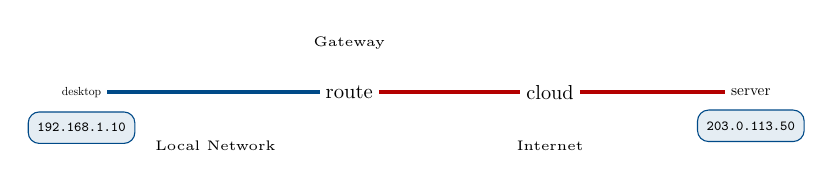
\begin{tikzpicture}[scale=0.85]
            % Source PC
            \node[pc] (pc1) at (0,0) {\iconpc[0.5cm]};
            \node[ipbox, below=0.1cm of pc1, font=\tiny\ttfamily] {192.168.1.10};
            
            % Router
            \node[router] (rtr) at (4,0) {\iconrouter[0.6cm]};
            \node[font=\tiny, above] at (4,0.5) {Gateway};
            
            % Cloud/Internet
            \node[cloud] (cloud) at (7,0) {\iconcloud[0.6cm]};
            
            % Destination server
            \node[server] (srv) at (10,0) {\iconserver[0.5cm]};
            \node[ipbox, below=0.1cm of srv, font=\tiny\ttfamily] {203.0.113.50};
            
            % Connections
            \draw[ethernet noarrow, line width=1.5pt] (pc1) -- (rtr);
            \draw[wan noarrow, line width=1.5pt] (rtr) -- (cloud);
            \draw[wan noarrow, line width=1.5pt] (cloud) -- (srv);
            
            % Labels
            \node[font=\tiny] at (2,-0.8) {Local Network};
            \node[font=\tiny] at (7,-0.8) {Internet};
        \end{tikzpicture}
    \end{center}

\articleonly{
\par\small\emph{This diagram illustrates the end-to-end journey of IP communication: a source PC (192.168.1.10) on a local network connects through a gateway router to the internet cloud, ultimately reaching a destination server (203.0.113.50) on a remote network. The local network uses Ethernet connections while internet traffic travels over WAN links, demonstrating how Layer 3 IP addressing enables communication across different network types and geographic locations.}\par
}

\end{frame}

% Table of contents in presentation mode only
\presentationonly{
\begin{frame}[allowframebreaks]{Outline}
\small
\tableofcontents[hideallsubsections]
\end{frame}
}


% =============================================================================
% SLIDE 2: Review - From Layer 2 to Layer 3
% =============================================================================
\section*{Review from Module 3}

\begin{frame}{Review: From Layer 2 to Layer 3}
    \begin{columns}[T]
        \begin{column}{0.55\textwidth}
            \begin{itemize}
                \item Module 3 covered \textbf{switches} and \textbf{MAC addresses} (Layer 2).
                \item Today's question: How do we communicate \textit{beyond} our local network?
                \item MAC addresses only work locally---switches don't forward to other networks.
                \item We need \keyterm{IP addresses} (Layer 3) to route traffic across networks.
            \end{itemize}
            
            \vspace{0.3em}
            \begin{alertblock}{The Key Difference}
                \textbf{MAC} = local delivery (within your network) \\
                \textbf{IP} = end-to-end delivery (across the internet)
            \end{alertblock}
        \end{column}
        \begin{column}{0.42\textwidth}
            \begin{center}
                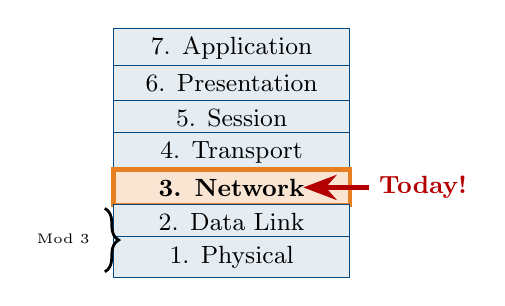
\begin{tikzpicture}[scale=0.7]
                    % OSI Stack
                    \node[osilayer] (l7) at (0, 3.15) {7. Application};
                    \node[osilayer] (l6) at (0, 2.52) {6. Presentation};
                    \node[osilayer] (l5) at (0, 1.89) {5. Session};
                    \node[osilayer] (l4) at (0, 1.26) {4. Transport};
                    \node[osilayer highlight] (l3) at (0, 0.63) {3. Network};
                    \node[osilayer] (l2) at (0, 0) {2. Data Link};
                    \node[osilayer] (l1) at (0, -0.63) {1. Physical};
                    
                    % Today's focus arrow
                    \draw[-{Stealth}, line width=2pt, alertred] (2.5, 0.63) -- (1.3, 0.63);
                    \node[right, font=\small\bfseries, alertred] at (2.5, 0.63) {Today!};
                    
                    % Module 3 bracket
                    \draw[decorate, decoration={brace, amplitude=5pt, mirror}, line width=1pt] 
                        (-2.3, -0.9) -- (-2.3, 0.25);
                    \node[left, font=\tiny] at (-2.4, -0.3) {Mod 3};
                \end{tikzpicture}
            \end{center}
        \end{column}
    \end{columns}
\end{frame}

% =============================================================================
% SLIDE 3: Learning Outcomes
% =============================================================================
\begin{frame}[t,allowframebreaks]{Learning Outcomes}
    After completing this module, you will be able to:
    \vspace{0.5em}
    \begin{itemize}
        \item Explain the role of \keyterm{Layer 3 (IP) addressing} and how it differs from Layer 2 (MAC) addressing.
        \item Describe \keyterm{ARP} (Address Resolution Protocol) and how it maps IP addresses to MAC addresses.
        \item Interpret \keyterm{IPv4 addresses} in dotted decimal notation and understand the role of \keyterm{subnet masks}.
        \item Calculate network addresses, broadcast addresses, and usable host ranges using \keyterm{CIDR notation}.
        \item Apply \keyterm{VLSM} (Variable Length Subnet Masking) to create subnets of different sizes.
        \item Identify \keyterm{private IP ranges} (RFC 1918) and explain \keyterm{NAT} (Network Address Translation).
        \item Configure IP addresses, subnet masks, and \keyterm{default gateways} on network devices.
        \item Use troubleshooting tools including \keyterm{ping}, \keyterm{arp}, \keyterm{ipconfig/ifconfig}, and \keyterm{traceroute}.
        \item Compare \keyterm{IPv4} and \keyterm{IPv6} addressing formats and describe IPv6 adoption strategies.
    \end{itemize}
\end{frame}



% =============================================================================
% SLIDE 5: The IPv4 Datagram Header
% =============================================================================
\section{IP Fundamentals and Address Resolution}
\subsection{IPv4 Header and Address Roles}

\articleonly{
This section introduces IPv4 packet structure and the relationship between Layer 2 and Layer 3 addressing during local delivery and routing.
}

\begin{frame}{The IPv4 Datagram Header}
    \begin{columns}[T]
        \begin{column}{0.48\textwidth}
            \begin{itemize}
                \item IP wraps data in a \keyterm{datagram} (like frames at Layer 2).
                \item Header contains addressing and control information.
                \item Key fields:
                    \begin{itemize}
                        \scriptsize
                        \item \textbf{Version}: 4 for IPv4
                        \item \textbf{TTL}: Time to Live (hop limit)
                        \item \textbf{Source IP}: Sender's address
                        \item \textbf{Destination IP}: Receiver's address
                        \item \textbf{Protocol}: What's inside (TCP, UDP)
                    \end{itemize}
            \end{itemize}
            
            \vspace{0.3em}
            \begin{alertblock}{TTL Prevents Loops}
                Each router decrements TTL by 1. When TTL reaches 0, the packet is discarded---prevents infinite loops!
            \end{alertblock}
        \end{column}
        \begin{column}{0.48\textwidth}
            \begin{center}
                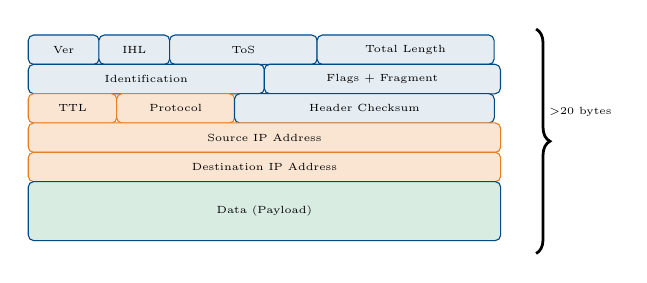
\begin{tikzpicture}[scale=0.75, transform shape]
                    % Header fields (simplified)
                    \node[pktseg, minimum width=1.2cm] (ver) at (0,0) {Ver};
                    \node[pktseg, minimum width=1.2cm, right=-0.5pt of ver] (ihl) {IHL};
                    \node[pktseg, minimum width=2.5cm, right=-0.5pt of ihl] (tos) {ToS};
                    \node[pktseg, minimum width=3cm, right=-0.5pt of tos] (len) {Total Length};
                    
                    % Row 2
                    \node[pktseg, minimum width=4cm, below=-0.5pt of ver.south west, anchor=north west] (id) {Identification};
                    \node[pktseg, minimum width=4cm, right=-0.5pt of id] (frag) {Flags + Fragment};
                    
                    % Row 3
                    \node[pktseg highlight, minimum width=1.5cm, below=-0.5pt of id.south west, anchor=north west] (ttl) {TTL};
                    \node[pktseg highlight, minimum width=2cm, right=-0.5pt of ttl] (proto) {Protocol};
                    \node[pktseg, minimum width=4.4cm, right=-0.5pt of proto] (chk) {Header Checksum};
                    
                    % Row 4 - Source IP
                    \node[pktseg highlight, minimum width=8cm, below=-0.5pt of ttl.south west, anchor=north west] (src) {Source IP Address};
                    
                    % Row 5 - Dest IP
                    \node[pktseg highlight, minimum width=8cm, below=-0.5pt of src.south west, anchor=north west] (dst) {Destination IP Address};
                    
                    % Data
                    \node[pktseg, minimum width=8cm, minimum height=1cm, below=-0.5pt of dst.south west, anchor=north west, fill=networkgreen!15] (data) {Data (Payload)};
                    
                    % Size annotation
                    \draw[decorate, decoration={brace, amplitude=5pt}, line width=1pt]
                        (8.0, 0.35) -- (8.0, -3.45);
                    \node[font=\tiny, right] at (8.1, -1.05) {>20 bytes};
                \end{tikzpicture}
            \end{center}

\articleonly{
\par\small\emph{This diagram shows the structure of an IPv4 packet header with key fields arranged in five rows: Row 1 contains Version and IHL (Internet Header Length) defining header format and size; Row 2 has DSCP for quality of service and Total Length for packet size; Row 3 includes Identification, Flags, and Fragment Offset for packet reassembly; Row 4 shows Time To Live (preventing infinite routing loops), Protocol (identifying upper layer like TCP/UDP), and Header Checksum for error detection; Rows 4-5 contain the critical Source IP Address and Destination IP Address fields that enable end-to-end routing. The entire header is at least 20 bytes before the data payload begins.}\par
}

        \end{column}
    \end{columns}
\end{frame}

% =============================================================================
% SLIDE 6: Layer 2 vs Layer 3 Addressing
% =============================================================================
\begin{frame}{Layer 2 vs Layer 3 Addressing}
    \begin{columns}[T]
        \begin{column}{0.48\textwidth}
            \begin{block}{MAC Address (Layer 2)}
                \begin{itemize}
                    \item Hardware address burned into NIC
                    \item Works only on \textbf{local network}
                    \item \textbf{Changes} at each router hop
                    \item Example: \texttt{00:1A:2B:3C:4D:5E}
                \end{itemize}
            \end{block}
            
            \vspace{0.3em}
            \begin{block}{IP Address (Layer 3)}
                \begin{itemize}
                    \item Logical address assigned by admin
                    \item Works \textbf{across networks}
                    \item \textbf{Stays the same} end-to-end
                    \item Example: \texttt{192.168.1.100}
                \end{itemize}
            \end{block}
        \end{column}
        \begin{column}{0.48\textwidth}
            \begin{exampleblock}{Mailing Analogy}
                \textbf{IP address} = Full mailing address \\
                (123 Main St, Springfield, USA)
                
                \vspace{0.3em}
                \textbf{MAC address} = Apartment number \\
                (Apt 4B---only meaningful inside the building)
            \end{exampleblock}
            
            \vspace{0.3em}
            \begin{center}
                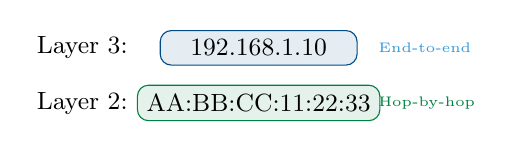
\begin{tikzpicture}[scale=0.7]
                    % Layer labels
                    \node[ipbox, minimum width=2.5cm] (ip) at (0,0) {192.168.1.10};
                    \node[font=\small, left] at (-2.2,0) {Layer 3:};
                    
                    \node[macbox, minimum width=2.5cm] (mac) at (0,-1) {AA:BB:CC:11:22:33};
                    \node[font=\small, left] at (-2.2,-1) {Layer 2:};
                    
                    % Annotations
                    \node[font=\tiny, right, ipblue] at (2,0) {End-to-end};
                    \node[font=\tiny, right, networkgreen] at (2,-1) {Hop-by-hop};
                \end{tikzpicture}
            \end{center}
        \end{column}
    \end{columns}
\end{frame}

% =============================================================================
% SLIDE 7: How Routers Use Both Addresses
% =============================================================================
\begin{frame}{How Routers Use Both Addresses}
    \begin{center}
        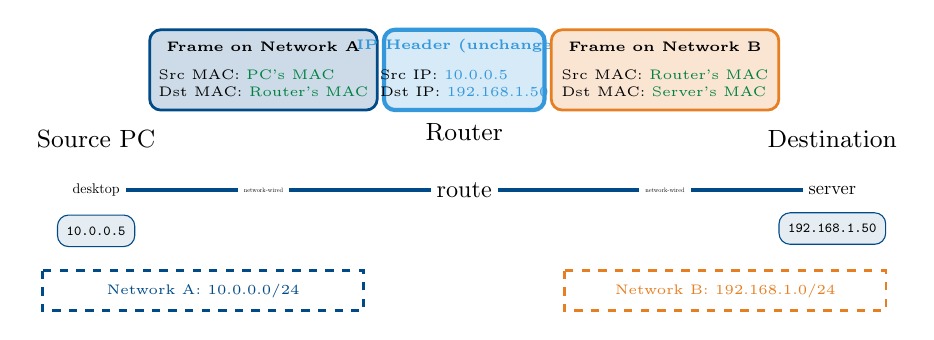
\begin{tikzpicture}[scale=0.85]
            % Network A
            \node[pc] (pc) at (0,0) {\iconpc[0.6cm]};
            \node[font=\small, above] at (0,0.5) {Source PC};
            \node[ipbox, below=0.15cm of pc, font=\tiny\ttfamily] (pcip) {10.0.0.5};
            
            % Switch A
            \node[switch] (sw1) at (2.5,0) {\iconswitch[0.5cm]};
            
            % Router
            \node[router] (rtr) at (5.5,0) {\iconrouter[0.7cm]};
            \node[font=\small, above] at (5.5,0.6) {Router};
            
            % Switch B
            \node[switch] (sw2) at (8.5,0) {\iconswitch[0.5cm]};
            
            % Server
            \node[server] (srv) at (11,0) {\iconserver[0.6cm]};
            \node[font=\small, above] at (11,0.5) {Destination};
            \node[ipbox, below=0.15cm of srv, font=\tiny\ttfamily] (srvip) {192.168.1.50};
            
            % Connections
            \draw[ethernet noarrow] (pc) -- (sw1);
            \draw[ethernet noarrow] (sw1) -- (rtr);
            \draw[ethernet noarrow] (rtr) -- (sw2);
            \draw[ethernet noarrow] (sw2) -- (srv);
            
            % Network labels
            \draw[dashed, rctcblue, line width=1pt] (-0.8,-1.2) rectangle (4,-1.8);
            \node[font=\tiny, rctcblue] at (1.6,-1.5) {Network A: 10.0.0.0/24};
            
            \draw[dashed, aborange, line width=1pt] (7,-1.2) rectangle (11.8,-1.8);
            \node[font=\tiny, aborange] at (9.4,-1.5) {Network B: 192.168.1.0/24};
            
            % Frame on Network A
            \draw[fill=rctcblue!20, draw=rctcblue, line width=1pt, rounded corners]
                (0.8,1.2) rectangle (4.2,2.4);
            \node[font=\tiny\bfseries] at (2.5,2.15) {Frame on Network A};
            \node[font=\tiny, align=left] at (2.5,1.6) {
                Src MAC: \textcolor{networkgreen}{PC's MAC} \\
                Dst MAC: \textcolor{networkgreen}{Router's MAC}
            };
            
            % IP stays same (shown in middle)
            \draw[fill=ipblue!20, draw=ipblue, line width=1.5pt, rounded corners]
                (4.3,1.2) rectangle (6.7,2.4);
            \node[font=\tiny\bfseries, ipblue] at (5.5,2.15) {IP Header (unchanged)};
            \node[font=\tiny, align=left] at (5.5,1.6) {
                Src IP: \textcolor{ipblue}{10.0.0.5} \\
                Dst IP: \textcolor{ipblue}{192.168.1.50}
            };
            
            % Frame on Network B
            \draw[fill=aborange!20, draw=aborange, line width=1pt, rounded corners]
                (6.8,1.2) rectangle (10.2,2.4);
            \node[font=\tiny\bfseries] at (8.5,2.15) {Frame on Network B};
            \node[font=\tiny, align=left] at (8.5,1.6) {
                Src MAC: \textcolor{networkgreen}{Router's MAC} \\
                Dst MAC: \textcolor{networkgreen}{Server's MAC}
            };
        \end{tikzpicture}
    \end{center}

\articleonly{
\par\small\emph{This complex diagram demonstrates how routers handle frame forwarding across network boundaries. A source PC (10.0.0.5) on Network A sends traffic through a switch to a router, which then forwards to Network B where the destination server (192.168.1.50) resides. Three boxed sections show the critical concept: on Network A, the frame's source MAC is the PC and destination MAC is the router; the middle IP header box (highlighted in blue) shows that source and destination IP addresses remain unchanged throughout the journey; on Network B, the router creates a new frame with its own MAC as source and the server's MAC as destination. This illustrates that Layer 2 MAC addresses change at each hop while Layer 3 IP addresses provide end-to-end addressing.}\par
}
    
    \vspace{0.2em}
    \begin{block}{Key Insight}
        \textbf{IP addresses} stay the same from source to destination. \textbf{MAC addresses} change at every hop---the router creates a new frame for each network segment.
    \end{block}
\end{frame}

% =============================================================================
% SLIDE 8: Address Resolution Protocol (ARP)
% =============================================================================
\begin{frame}{Address Resolution Protocol (ARP)}
    \begin{columns}[T]
        \begin{column}{0.48\textwidth}
            \begin{itemize}
                \item Problem: You know the \textbf{destination IP}, but need the \textbf{MAC} to send a frame.
                \item Solution: \keyterm{ARP} asks ``Who has this IP?''
                \item ARP Request: Broadcast to all devices---``Who has 192.168.1.50?''
                \item ARP Reply: Target responds with its MAC address (unicast).
                \item Result is cached in the \keyterm{ARP table}.
            \end{itemize}
            
            \vspace{0.3em}
            \begin{alertblock}{Security Note}
                ARP has no authentication. \textbf{ARP spoofing} attacks send fake replies to redirect traffic!
            \end{alertblock}
        \end{column}
        \begin{column}{0.48\textwidth}
            \begin{center}
                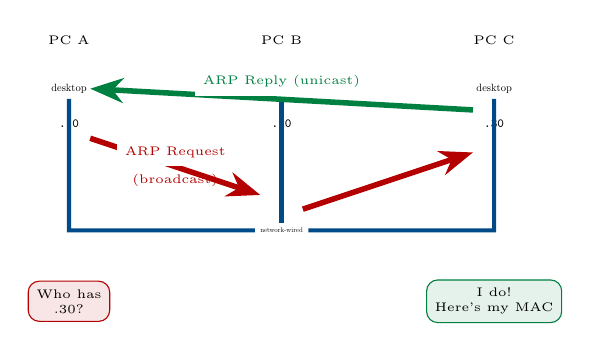
\begin{tikzpicture}[scale=0.9, transform shape]
                    % Devices
                    \node[pc] (pc1) at (0,2.5) {\iconpc[0.5cm]};
                    \node[font=\tiny, above] at (0,3) {PC A};
                    \node[font=\tiny\ttfamily] at (0,2) {.10};
                    
                    \node[pc] (pc2) at (3,2.5) {\iconpc[0.5cm]};
                    \node[font=\tiny, above] at (3,3) {PC B};
                    \node[font=\tiny\ttfamily] at (3,2) {.20};
                    
                    \node[pc] (pc3) at (6,2.5) {\iconpc[0.5cm]};
                    \node[font=\tiny, above] at (6,3) {PC C};
                    \node[font=\tiny\ttfamily] at (6,2) {.30};
                    
                    % Switch
                    \node[switch] (sw) at (3,0.5) {\iconswitch[0.6cm]};
                    
                    % Connections
                    \draw[ethernet noarrow] (pc1) -- (0,0.5) -- (sw);
                    \draw[ethernet noarrow] (pc2) -- (sw);
                    \draw[ethernet noarrow] (pc3) -- (6,0.5) -- (sw);
                    
                    % ARP Request (broadcast)
                    \draw[-{Stealth}, alertred, line width=2pt] (0.3,1.8) -- (2.7,1.0);
                    \draw[-{Stealth}, alertred, line width=2pt] (3.3,0.8) -- (5.7,1.6);
                    \node[font=\tiny, alertred, fill=white] at (1.5,1.6) {ARP Request};
                    \node[font=\tiny, alertred] at (1.5,1.2) {(broadcast)};
                    
                    % ARP Reply (unicast)
                    \draw[-{Stealth}, networkgreen, line width=2pt] (5.7,2.2) -- (0.3,2.5);
                    \node[font=\tiny, networkgreen, fill=white] at (3,2.6) {ARP Reply (unicast)};
                    
                    % Question/Answer
                    \node[font=\tiny, align=center, fill=alertred!10, draw=alertred, rounded corners] 
                        at (0,-0.5) {Who has\\.30?};
                    \node[font=\tiny, align=center, fill=networkgreen!10, draw=networkgreen, rounded corners] 
                        at (6,-0.5) {I do!\\Here's my MAC};
                \end{tikzpicture}
            \end{center}
        \end{column}
    \end{columns}
\end{frame}

% =============================================================================
% SLIDE 9: ARP Table and Cache
% =============================================================================
\begin{frame}{ARP Table and Cache}
    \begin{columns}[T]
        \begin{column}{0.48\textwidth}
            \begin{itemize}
                \item ARP results are stored in the \keyterm{ARP cache} (also called ARP table).
                \item Avoids broadcasting for every single packet.
                \item Entries expire after a timeout (typically 2--20 minutes).
                \item View with: \texttt{arp -a} (Windows/Linux/Mac)
            \end{itemize}
            
            \vspace{0.3em}
            \begin{block}{Common ARP Commands}
                \small
                \texttt{arp -a} --- Display all entries \\
                \texttt{arp -d [IP]} --- Delete an entry \\
                \texttt{arp -s [IP] [MAC]} --- Add static entry
            \end{block}
        \end{column}
        \begin{column}{0.48\textwidth}
            \begin{block}{Sample ARP Table Output}
                \ttfamily\small
                \begin{tabular}{l l}
                    \textbf{IP Address} & \textbf{MAC Address} \\
                    \midrule
                    192.168.1.1 & 00:1a:2b:3c:4d:01 \\
                    192.168.1.25 & 00:1a:2b:3c:4d:25 \\
                    192.168.1.50 & 00:1a:2b:3c:4d:50 \\
                \end{tabular}
            \end{block}
            
            \vspace{0.3em}
            \begin{alertblock}{Troubleshooting Tip}
                Empty ARP table? No local communication is happening---check Layer 1 and 2 first!
            \end{alertblock}
        \end{column}
    \end{columns}
\end{frame}

% =============================================================================
% SLIDE 10: Unicast, Broadcast, Multicast, and Anycast
% =============================================================================
\begin{frame}{Unicast, Broadcast, Multicast, and Anycast}
    \begin{center}
        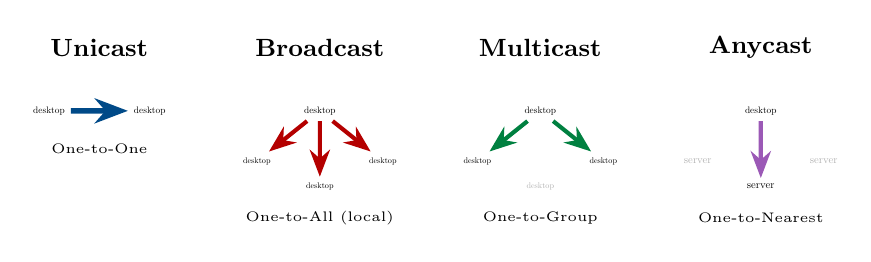
\begin{tikzpicture}[scale=0.8]
            % === UNICAST ===
            \node[font=\small\bfseries] at (0,2.8) {Unicast};
            \node[pc] (u1) at (-0.8,1.8) {\iconpc[0.4cm]};
            \node[pc] (u2) at (0.8,1.8) {\iconpc[0.4cm]};
            \draw[-{Stealth}, rctcblue, line width=2pt] (u1) -- (u2);
            \node[font=\tiny] at (0,1.2) {One-to-One};
            
            % === BROADCAST ===
            \node[font=\small\bfseries] at (3.5,2.8) {Broadcast};
            \node[pc] (b1) at (3.5,1.8) {\iconpc[0.4cm]};
            \node[pc] (b2) at (2.5,1.0) {\iconpc[0.35cm]};
            \node[pc] (b3) at (3.5,0.6) {\iconpc[0.35cm]};
            \node[pc] (b4) at (4.5,1.0) {\iconpc[0.35cm]};
            \draw[-{Stealth}, alertred, line width=1.5pt] (b1) -- (b2);
            \draw[-{Stealth}, alertred, line width=1.5pt] (b1) -- (b3);
            \draw[-{Stealth}, alertred, line width=1.5pt] (b1) -- (b4);
            \node[font=\tiny] at (3.5,0.1) {One-to-All (local)};
            
            % === MULTICAST ===
            \node[font=\small\bfseries] at (7,2.8) {Multicast};
            \node[pc] (m1) at (7,1.8) {\iconpc[0.4cm]};
            \node[pc] (m2) at (6,1.0) {\iconpc[0.35cm]};
            \node[pc, opacity=0.3] (m3) at (7,0.6) {\iconpc[0.35cm]};
            \node[pc] (m4) at (8,1.0) {\iconpc[0.35cm]};
            \draw[-{Stealth}, networkgreen, line width=1.5pt] (m1) -- (m2);
            \draw[-{Stealth}, networkgreen, line width=1.5pt] (m1) -- (m4);
            \node[font=\tiny] at (7,0.1) {One-to-Group};
            
            % === ANYCAST ===
            \node[font=\small\bfseries] at (10.5,2.8) {Anycast};
            \node[pc] (a1) at (10.5,1.8) {\iconpc[0.4cm]};
            \node[server, opacity=0.3] (a2) at (9.5,1.0) {\iconserver[0.35cm]};
            \node[server] (a3) at (10.5,0.6) {\iconserver[0.35cm]};
            \node[server, opacity=0.3] (a4) at (11.5,1.0) {\iconserver[0.35cm]};
            \draw[-{Stealth}, ippurple, line width=1.5pt] (a1) -- (a3);
            \node[font=\tiny] at (10.5,0.1) {One-to-Nearest};
        \end{tikzpicture}
    \end{center}
    
    \vspace{0.3em}
    \begin{columns}[T]
        \begin{column}{0.48\textwidth}
            \begin{block}{Common Uses}
                \small
                \textbf{Unicast}: Most traffic (web, email) \\
                \textbf{Broadcast}: ARP, DHCP discovery
            \end{block}
        \end{column}
        \begin{column}{0.48\textwidth}
            \begin{block}{Common Uses}
                \small
                \textbf{Multicast}: Video streaming, routing updates \\
                \textbf{Anycast}: DNS, CDNs (find closest server)
            \end{block}
        \end{column}
    \end{columns}
\end{frame}

% =============================================================================
% SLIDE 11: Case Study - Homer's Home Network Mystery
% =============================================================================
\begin{frame}{Case Study: Homer's Home Network Mystery}
    \begin{casestudy}{Homer's Home Network Mystery}
        Homer Simpson just set up a new PC in his home office. He runs some tests:
        
        \vspace{0.5em}
        \begin{itemize}
            \item He can ping \texttt{127.0.0.1} (loopback) --- \textcolor{networkgreen}{Success!}
            \item He can ping his own IP \texttt{192.168.1.50} --- \textcolor{networkgreen}{Success!}
            \item He \textbf{cannot} ping Marge's laptop \texttt{192.168.1.51} --- \textcolor{alertred}{Fails!}
            \item He \textbf{cannot} reach the internet --- \textcolor{alertred}{Fails!}
        \end{itemize}
        
        \vspace{0.5em}
        Homer runs \texttt{arp -a} and sees an \textbf{empty ARP table}.
    \end{casestudy}
    
    \begin{block}{Review Questions}
        \begin{enumerate}
            \item What does an empty ARP table suggest about network communication?
            \item What Layer 1 or Layer 2 issue might cause this?
            \item What should Homer check first?
        \end{enumerate}
    \end{block}
\end{frame}

% =============================================================================
% SLIDE 12: Case Study Solution - Homer's Home Network Mystery
% =============================================================================
\begin{frame}{Case Study Solution: Homer's Home Network Mystery}
    \begin{casesolution}{Homer's Home Network Mystery}
        \begin{enumerate}
            \item Empty ARP table means \textbf{no successful local communication}---ARP requests aren't being answered (or sent).
            \item Likely Layer 1/2 causes:
                \begin{itemize}
                    \scriptsize
                    \item Ethernet cable unplugged or damaged
                    \item NIC disabled in operating system
                    \item Switch port is dead or disabled
                    \item Wrong VLAN assignment on switch port
                \end{itemize}
            \item Homer should check (in order):
                \begin{itemize}
                    \scriptsize
                    \item Cable connection at PC and switch
                    \item Link lights on NIC and switch port
                    \item NIC status in Windows (Network Connections)
                \end{itemize}
        \end{enumerate}
    \end{casesolution}
    
    \vspace{0.3em}
    \begin{alertblock}{Key Lesson}
        \scriptsize
        If the ARP table is empty, the problem is almost always \textbf{Layer 1 or Layer 2}---not the IP configuration. Check physical connectivity first!
    \end{alertblock}
\end{frame}

% =============================================================================
% SLIDE 13: IPv4 Address Format
% =============================================================================
\section{Subnetting and Host Addressing}
\subsection{Address Structure and Masks}

\articleonly{
This section covers IPv4 addressing structure, subnet masks, and host range calculations used in practical network design.
}

\begin{frame}{IPv4 Address Format}
    \begin{columns}[T]
        \begin{column}{0.52\textwidth}
            \begin{itemize}
                \item IPv4 addresses are \textbf{32 bits} long.
                \item Written as four \keyterm{octets} in decimal, separated by dots.
                \item Each octet ranges from \textbf{0 to 255}.
                \item Total possible addresses: about 4.3 billion.
                \item Not enough for today's internet!
            \end{itemize}
            
            \vspace{0.3em}
            \begin{alertblock}{Why 0--255?}
                Each octet is 8 bits. $2^8 = 256$ possible values (0 through 255).
            \end{alertblock}
        \end{column}
        \begin{column}{0.45\textwidth}
            \begin{center}
                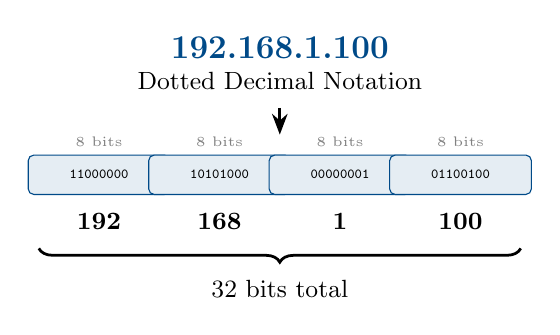
\begin{tikzpicture}[scale=0.85]
                    % Decimal representation
                    \node[font=\large\bfseries, rctcblue] at (0,3.5) {192.168.1.100};
                    \node[font=\small] at (0,3) {Dotted Decimal Notation};
                    
                    % Arrow down
                    \draw[-{Stealth}, line width=1pt] (0,2.6) -- (0,2.2);
                    
                    % Binary boxes - spread out more
                    \node[pktseg, minimum width=1.8cm, font=\tiny\ttfamily] (b1) at (-2.7,1.6) {11000000};
                    \node[pktseg, minimum width=1.8cm, font=\tiny\ttfamily] (b2) at (-0.9,1.6) {10101000};
                    \node[pktseg, minimum width=1.8cm, font=\tiny\ttfamily] (b3) at (0.9,1.6) {00000001};
                    \node[pktseg, minimum width=1.8cm, font=\tiny\ttfamily] (b4) at (2.7,1.6) {01100100};
                    
                    % Decimal values below - with more space
                    \node[font=\small\bfseries] at (-2.7,0.9) {192};
                    \node[font=\small\bfseries] at (-0.9,0.9) {168};
                    \node[font=\small\bfseries] at (0.9,0.9) {1};
                    \node[font=\small\bfseries] at (2.7,0.9) {100};
                    
                    % 8 bits labels above each box
                    \node[font=\tiny, gray] at (-2.7,2.1) {8 bits};
                    \node[font=\tiny, gray] at (-0.9,2.1) {8 bits};
                    \node[font=\tiny, gray] at (0.9,2.1) {8 bits};
                    \node[font=\tiny, gray] at (2.7,2.1) {8 bits};
                    
                    % Bit count brace at bottom
                    \draw[decorate, decoration={brace, amplitude=5pt, mirror}, line width=1pt]
                        (-3.6,0.5) -- (3.6,0.5);
                    \node[font=\small] at (0,-0.1) {32 bits total};
                \end{tikzpicture}
            \end{center}

\articleonly{
\par\small\emph{This diagram breaks down the IPv4 address 192.168.1.100 into its binary representation, showing four octets (8-bit segments): 11000000 (192), 10101000 (168), 00000001 (1), and 01100100 (100). Each octet is labeled "8 bits" above, and a brace below indicates the total address is 32 bits. This binary-to-decimal conversion is fundamental to understanding IP addressing, subnetting, and how network masks work at the bit level to separate network and host portions.}\par
}

        \end{column}
    \end{columns}
\end{frame}

% =============================================================================
% SLIDE 14: Network Masks Explained
% =============================================================================
\begin{frame}{Network Masks Explained}
    \begin{columns}[T]
        \begin{column}{0.40\textwidth}
            \begin{itemize}
                \item Every IP address has two parts:
                    \begin{itemize}
                        \item \textbf{Network portion}: Which network?
                        \item \textbf{Host portion}: Which device?
                    \end{itemize}
                \item The \keyterm{subnet mask} defines where to split.
                \item Mask uses \textbf{1s} for network bits, \textbf{0s} for host bits.
            \end{itemize}
            
            \vspace{0.3em}
            \begin{exampleblock}{Analogy}
                Think of a phone number: area code (network) + local number (host).
            \end{exampleblock}
        \end{column}
        \begin{column}{0.60\textwidth}
            \begin{center}
                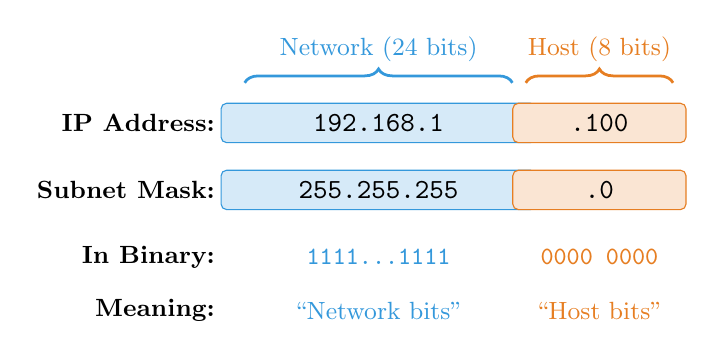
\begin{tikzpicture}[scale=0.85]
                    % Network portion label at top
                    \draw[decorate, decoration={brace, amplitude=5pt}, line width=1pt, ipblue]
                        (-3.2,3.8) -- (0.8,3.8);
                    \node[font=\small, ipblue] at (-1.2,4.3) {Network (24 bits)};
                    
                    % Host portion label at top
                    \draw[decorate, decoration={brace, amplitude=5pt}, line width=1pt, aborange]
                        (1.0,3.8) -- (3.2,3.8);
                    \node[font=\small, aborange] at (2.1,4.3) {Host (8 bits)};
                    
                    % IP Address row
                    \node[font=\small\bfseries, left] at (-3.5,3.2) {IP Address:};
                    \node[pktseg highlight, minimum width=4cm, font=\normalsize\ttfamily, fill=ipblue!20, draw=ipblue] (ip1) at (-1.2,3.2) {192.168.1};
                    \node[pktseg, minimum width=2.2cm, font=\normalsize\ttfamily, fill=aborange!20, draw=aborange] (ip2) at (2.1,3.2) {.100};
                    
                    % Subnet Mask row
                    \node[font=\small\bfseries, left] at (-3.5,2.2) {Subnet Mask:};
                    \node[pktseg, minimum width=4cm, font=\normalsize\ttfamily, fill=ipblue!20, draw=ipblue] (m1) at (-1.2,2.2) {255.255.255};
                    \node[pktseg, minimum width=2.2cm, font=\normalsize\ttfamily, fill=aborange!20, draw=aborange] (m2) at (2.1,2.2) {.0};
                    
                    % Binary explanation row
                    \node[font=\small\bfseries, left] at (-3.5,1.2) {In Binary:};
                    \node[font=\small\ttfamily, ipblue] at (-1.2,1.2) {1111...1111};
                    \node[font=\small\ttfamily, aborange] at (2.1,1.2) {0000 0000};
                    
                    % Meaning row
                    \node[font=\small\bfseries, left] at (-3.5,0.4) {Meaning:};
                    \node[font=\small, ipblue] at (-1.2,0.4) {``Network bits''};
                    \node[font=\small, aborange] at (2.1,0.4) {``Host bits''};
                \end{tikzpicture}
            \end{center}
        \end{column}
    \end{columns}
\end{frame}


% =============================================================================
% SLIDE 15: Subnet Mask Examples
% =============================================================================
\begin{frame}[t,shrink=15]{Subnet Mask Examples}
    \begin{center}
        \begin{tabular}{l c c c}
            \toprule
            \textbf{Subnet Mask} & \textbf{CIDR} & \textbf{Total Addresses} & \textbf{Usable Hosts} \\
            \midrule
            255.0.0.0 & /8 & 16,777,216 & 16,777,214 \\
            255.255.0.0 & /16 & 65,536 & 65,534 \\
            \rowcolor{rctcblue!10}
            255.255.255.0 & /24 & 256 & 254 \\
            255.255.255.128 & /25 & 128 & 126 \\
            255.255.255.192 & /26 & 64 & 62 \\
            255.255.255.224 & /27 & 32 & 30 \\
            255.255.255.240 & /28 & 16 & 14 \\
            255.255.255.248 & /29 & 8 & 6 \\
            255.255.255.252 & /30 & 4 & 2 \\
            \bottomrule
        \end{tabular}
    \end{center}
    
    \vspace{0.3em}
    \begin{columns}[T]
        \begin{column}{0.48\textwidth}
            \begin{block}{Why ``Usable'' Is Less}
                Two addresses are always reserved:
                \begin{itemize}
                    \item \textbf{Network address} -- all 0s in host portion
                    \item \textbf{Broadcast address} -- all 1s in host portion
                \end{itemize}
            \end{block}
        \end{column}
        \begin{column}{0.48\textwidth}
            \begin{exampleblock}{Formula}
                Usable hosts $= 2^{n} - 2$
                
                where $n$ = number of host bits
                
                \vspace{0.2em}
                Example: /24 has 8 host bits \\
                $2^{8} - 2 = 256 - 2 = 254$ hosts
            \end{exampleblock}
        \end{column}
    \end{columns}
\end{frame}

% =============================================================================
% SLIDE 16: Calculating Host Address Ranges
% =============================================================================
\begin{frame}{Calculating Host Address Ranges}
    \begin{columns}[T]
        \begin{column}{0.42\textwidth}
            \begin{block}{Given Information}
                \begin{itemize}
                    \item Network: \texttt{192.168.1.0/24}
                    \item Subnet Mask: \texttt{255.255.255.0}
                \end{itemize}
            \end{block}
            
            \vspace{0.3em}
            \begin{block}{Step-by-Step Calculation}
                \small
                \textbf{1. Network Address}: \\
                \quad \texttt{192.168.1.0} -- host bits all 0
                
                \vspace{0.2em}
                \textbf{2. First Usable Host}: \\
                \quad \texttt{192.168.1.1} -- network + 1
                
                \vspace{0.2em}
                \textbf{3. Last Usable Host}: \\
                \quad \texttt{192.168.1.254} -- broadcast - 1
                
                \vspace{0.2em}
                \textbf{4. Broadcast Address}: \\
                \quad \texttt{192.168.1.255} -- host bits all 1
            \end{block}
        \end{column}
        \begin{column}{0.55\textwidth}
            \begin{center}
                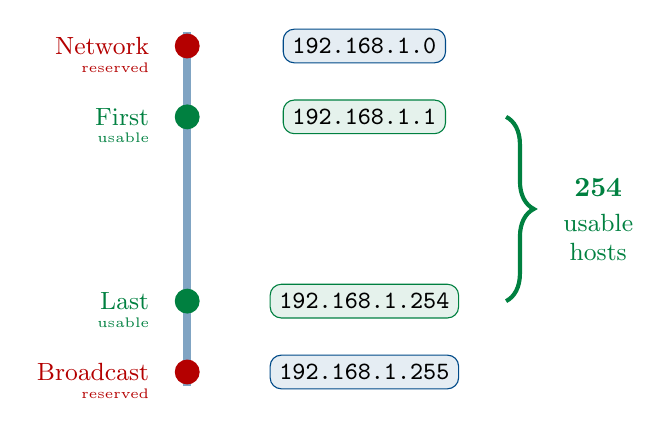
\begin{tikzpicture}[scale=0.9]
                    % Vertical line
                    \draw[line width=3pt, rctcblue!50] (0,0) -- (0,5);
                    
                    % Network address - top
                    \fill[alertred] (0,4.8) circle (5pt);
                    \node[ipbox, font=\small\ttfamily] at (2.5,4.8) {192.168.1.0};
                    \node[font=\small, alertred, align=right, anchor=east] at (-0.4,4.8) {Network};
                    \node[font=\tiny, alertred, anchor=east] at (-0.4,4.5) {reserved};
                    
                    % First usable
                    \fill[networkgreen] (0,3.8) circle (5pt);
                    \node[ipbox, font=\small\ttfamily, draw=networkgreen, fill=networkgreen!10] at (2.5,3.8) {192.168.1.1};
                    \node[font=\small, networkgreen, align=right, anchor=east] at (-0.4,3.8) {First};
                    \node[font=\tiny, networkgreen, anchor=east] at (-0.4,3.5) {usable};
                    
                    % Usable range indicator
                    \draw[decorate, decoration={brace, amplitude=10pt}, line width=1.5pt, networkgreen]
                        (4.5,3.8) -- (4.5,1.2);
                    \node[font=\normalsize\bfseries, networkgreen] at (5.8,2.8) {254};
                    \node[font=\small, networkgreen] at (5.8,2.3) {usable};
                    \node[font=\small, networkgreen] at (5.8,1.9) {hosts};
                    
                    % Last usable
                    \fill[networkgreen] (0,1.2) circle (5pt);
                    \node[ipbox, font=\small\ttfamily, draw=networkgreen, fill=networkgreen!10] at (2.5,1.2) {192.168.1.254};
                    \node[font=\small, networkgreen, align=right, anchor=east] at (-0.4,1.2) {Last};
                    \node[font=\tiny, networkgreen, anchor=east] at (-0.4,0.9) {usable};
                    
                    % Broadcast - bottom
                    \fill[alertred] (0,0.2) circle (5pt);
                    \node[ipbox, font=\small\ttfamily] at (2.5,0.2) {192.168.1.255};
                    \node[font=\small, alertred, align=right, anchor=east] at (-0.4,0.2) {Broadcast};
                    \node[font=\tiny, alertred, anchor=east] at (-0.4,-0.1) {reserved};
                \end{tikzpicture}
            \end{center}

\articleonly{
\par\small\emph{This vertical diagram illustrates the address allocation within subnet 192.168.1.0/24, showing five critical addresses from top to bottom: the network address (192.168.1.0, marked in red as reserved), the first usable host address (192.168.1.1, in green), a large green brace spanning to indicate 254 usable host addresses in the middle range, the last usable host address (192.168.1.254, in green), and the broadcast address (192.168.1.255, marked in red as reserved). This visualization demonstrates that in a /24 subnet, the first and last addresses are reserved for network identification and broadcasting, leaving 254 addresses available for host assignment.}\par
}

        \end{column}
    \end{columns}
\end{frame}

% =============================================================================
% SLIDE 17: Default Gateway
% =============================================================================
\begin{frame}{Default Gateway}
    \begin{columns}[T]
        \begin{column}{0.48\textwidth}
            \begin{itemize}
                \item The \keyterm{default gateway} is the router that connects your network to other networks.
                \item If destination IP is NOT on your local subnet $\rightarrow$ send to the gateway.
                \item Gateway must be on the \textbf{same subnet} as the host.
                \item Typically the first or last usable address (e.g., \texttt{.1} or \texttt{.254}).
            \end{itemize}
            
            \vspace{0.3em}
            \begin{alertblock}{Common Mistake}
                If the gateway is on a different subnet than the host, the host cannot reach it---and cannot reach anything outside the local network!
            \end{alertblock}
        \end{column}
        \begin{column}{0.48\textwidth}
            \begin{center}
                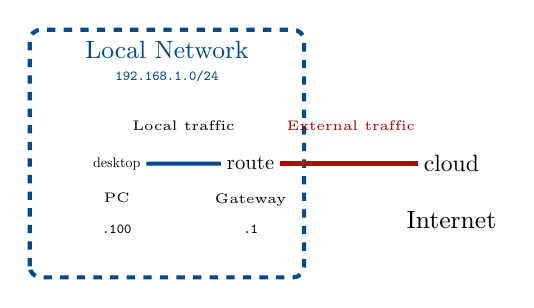
\begin{tikzpicture}[scale=0.85]
                    % Local network box
                    \draw[dashed, rctcblue, line width=1.5pt, rounded corners] 
                        (-0.8,-0.5) rectangle (3.3,3.2);
                    \node[font=\small, rctcblue] at (1.25,2.9) {Local Network};
                    \node[font=\tiny\ttfamily, rctcblue] at (1.25,2.5) {192.168.1.0/24};
                    
                    % PC
                    \node[pc] (pc) at (0.5,1.2) {\iconpc[0.6cm]};
                    \node[font=\tiny, below=0.1cm of pc] {PC};
                    \node[font=\tiny\ttfamily, below=0.5cm of pc] {.100};
                    
                    % Router (gateway)
                    \node[router] (rtr) at (2.5,1.2) {\iconrouter[0.6cm]};
                    \node[font=\tiny, below=0.1cm of rtr] {Gateway};
                    \node[font=\tiny\ttfamily, below=0.5cm of rtr] {.1};
                    
                    % Connection inside network
                    \draw[ethernet noarrow, line width=1.5pt] (pc) -- (rtr);
                    
                    % Internet cloud
                    \node[cloud] (cloud) at (5.5,1.2) {\iconcloud[0.7cm]};
                    \node[font=\small, below=0.3cm of cloud] {Internet};
                    
                    % Connection to internet
                    \draw[wan noarrow, line width=2pt] (rtr) -- (cloud);
                    
                    % Flow labels
                    \node[font=\tiny, above=0.3cm of {(1.5,1.2)}] {Local traffic};
                    \node[font=\tiny, above=0.3cm of {(4,1.2)}, alertred] {External traffic};
                \end{tikzpicture}
            \end{center}

\articleonly{
\par\small\emph{This diagram illustrates the default gateway concept within a local network (192.168.1.0/24) enclosed in a blue dashed box. A PC (.100) connects via Ethernet to a gateway router (.1), which in turn connects to the internet cloud via a WAN link. The arrows show local traffic staying within the network and external traffic passing through the gateway. The configuration block shows the PC's complete network settings: IP address 192.168.1.100, subnet mask 255.255.255.0, and critically, the gateway address 192.168.1.1 which must be on the same subnet as the host to be reachable.}\par
}
            
            \vspace{0.3em}
            \begin{block}{PC Configuration}
                \small
                IP: \texttt{192.168.1.100} \\
                Mask: \texttt{255.255.255.0} \\
                Gateway: \texttt{192.168.1.1}
            \end{block}
        \end{column}
    \end{columns}
\end{frame}

% =============================================================================
% SLIDE 18: Case Study - Moe's Tavern Network Problem
% =============================================================================
\begin{frame}{Case Study: Moe's Tavern Network Problem}
    \begin{casestudy}{Moe's Tavern Network Problem}
        Moe is setting up a new point-of-sale (POS) system at the tavern to track Duff Beer sales. The system is configured as follows:
        
        \vspace{0.5em}
        \begin{center}
            \scriptsize
            \begin{tabular}{l l}
                \textbf{Setting} & \textbf{Value} \\
                \midrule
                IP Address & \texttt{192.168.10.50} \\
                Subnet Mask & \texttt{255.255.255.0} \\
                Default Gateway & \texttt{192.168.20.1} \\
            \end{tabular}
        \end{center}
        
        Barney's laptop (\texttt{192.168.10.25}) can ping the POS system just fine. However, the POS system \textbf{cannot} reach the internet or the beer distributor's ordering website.
    \end{casestudy}
    
    \begin{block}{Review Questions}
        \begin{enumerate}
            \small
            \item What's wrong with this configuration?
            \item Why can Barney reach the POS but the POS can't reach the internet?
            \item What should the gateway address be?
        \end{enumerate}
    \end{block}
\end{frame}

% =============================================================================
% SLIDE 19: Case Study Solution - Moe's Tavern Network Problem
% =============================================================================
\begin{frame}{Case Study Solution: Moe's Tavern Network Problem}
    \begin{casesolution}{Moe's Tavern Network Problem}
        \begin{enumerate}
            \item The gateway \texttt{192.168.20.1} is on a \textbf{different subnet} than the POS system (\texttt{192.168.10.x}).
            \item Why Barney can reach POS but POS can't reach internet:
                \begin{itemize}
                    \item Barney and POS are on the \textbf{same subnet}---local traffic doesn't need the gateway
                    \item Internet traffic requires the gateway, which is \textbf{unreachable} (different subnet)
                \end{itemize}
            \item Gateway should be on the same subnet, such as \texttt{192.168.10.1}.
        \end{enumerate}
    \end{casesolution}
    
    \vspace{0.3em}
    \begin{center}
        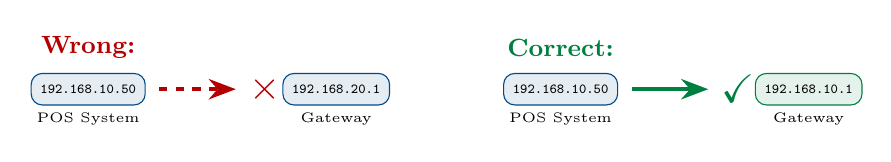
\begin{tikzpicture}[scale=0.75]
            % Wrong configuration
            \node[font=\small\bfseries, alertred] at (-3,1.5) {Wrong:};
            \node[ipbox, font=\tiny\ttfamily] at (-3,0.8) {192.168.10.50};
            \node[font=\tiny] at (-3,0.3) {POS System};
            
            \draw[-{Stealth}, alertred, line width=1.5pt, dashed] (-1.8,0.8) -- (-0.5,0.8);
            \node[font=\Large, alertred] at (0,0.8) {$\times$};
            
            \node[ipbox, font=\tiny\ttfamily] at (1.2,0.8) {192.168.20.1};
            \node[font=\tiny] at (1.2,0.3) {Gateway};
            
            % Right configuration
            \node[font=\small\bfseries, networkgreen] at (5,1.5) {Correct:};
            \node[ipbox, font=\tiny\ttfamily] at (5,0.8) {192.168.10.50};
            \node[font=\tiny] at (5,0.3) {POS System};
            
            \draw[-{Stealth}, networkgreen, line width=1.5pt] (6.2,0.8) -- (7.5,0.8);
            \node[font=\Large, networkgreen] at (8,0.8) {\checkmark};
            
            \node[ipbox, font=\tiny\ttfamily, draw=networkgreen, fill=networkgreen!10] at (9.2,0.8) {192.168.10.1};
            \node[font=\tiny] at (9.2,0.3) {Gateway};
        \end{tikzpicture}
    \end{center}

\articleonly{
\par\small\emph{This comparison diagram shows a common misconfiguration scenario on the left (marked "Wrong" in red) where a POS system at 192.168.10.50 tries to use gateway 192.168.20.1 on a different subnet, indicated by a dashed arrow and X symbol showing the unreachable gateway. The right side (marked "Correct" in green) shows the proper configuration where the same POS system uses gateway 192.168.10.1 on the same subnet, marked with a checkmark. This illustrates the critical requirement that default gateways must reside on the same subnet as the hosts they serve.}\par
}
    
    \vspace{0.2em}
    \begin{alertblock}{Key Lesson}
        The default gateway \textbf{must} be on the same subnet as the host. This is one of the most common misconfigurations!
    \end{alertblock}
\end{frame}

% =============================================================================
% SLIDE 20: Classful Addressing (Legacy)
% =============================================================================
\section{Address Planning Strategies}
\subsection{Classful, CIDR, and VLSM}

\articleonly{
Address planning evolved from classful limits to CIDR and VLSM for efficient allocation and scalable route summarization.
}

\begin{frame}{Classful Addressing (Legacy)}
    \begin{itemize}
        \item The original IP design divided addresses into \textbf{classes} based on the first octet.
        \item Each class had a fixed network/host boundary---no flexibility!
    \end{itemize}
    
    \vspace{0.3em}
    \begin{center}
        \begin{tabular}{l c c c c}
            \toprule
            \textbf{Class} & \textbf{First Octet} & \textbf{Default Mask} & \textbf{Networks} & \textbf{Hosts/Network} \\
            \midrule
            \rowcolor{ipblue!15}
            A & 1--126 & 255.0.0.0 (/8) & 126 & 16,777,214 \\
            \rowcolor{networkgreen!15}
            B & 128--191 & 255.255.0.0 (/16) & 16,384 & 65,534 \\
            \rowcolor{aborange!15}
            C & 192--223 & 255.255.255.0 (/24) & 2,097,152 & 254 \\
            D & 224--239 & \multicolumn{3}{c}{(Multicast---not for hosts)} \\
            E & 240--255 & \multicolumn{3}{c}{(Experimental---reserved)} \\
            \bottomrule
        \end{tabular}
    \end{center}
    
    \vspace{0.3em}
    \begin{columns}[T]
        \begin{column}{0.48\textwidth}
            \begin{alertblock}{The Problem}
                Very wasteful! A company needing 300 hosts had to get a Class B (65,534 addresses).
            \end{alertblock}
        \end{column}
        \begin{column}{0.48\textwidth}
            \begin{exampleblock}{The Solution}
                \keyterm{CIDR} (Classless Inter-Domain Routing) replaced classes with flexible prefix lengths.
            \end{exampleblock}
        \end{column}
    \end{columns}
\end{frame}

% =============================================================================
% SLIDE 21: Public vs Private Addressing
% =============================================================================
\begin{frame}{Public vs Private Addressing}
    \begin{columns}[T]
        \begin{column}{0.48\textwidth}
            \begin{block}{Public IP Addresses}
                \begin{itemize}
                    \item Routable on the internet
                    \item Must be globally unique
                    \item Assigned by ISPs (from IANA/RIRs)
                    \item Limited supply (IPv4 exhaustion!)
                \end{itemize}
            \end{block}
            
            \vspace{0.3em}
            \begin{block}{Private IP Addresses}
                \begin{itemize}
                    \item For internal networks only
                    \item \textbf{NOT} routable on internet
                    \item Can be reused by any organization
                    \item Free to use---no registration needed
                \end{itemize}
            \end{block}
        \end{column}
        \begin{column}{0.48\textwidth}
            \begin{alertblock}{Private Address Ranges}
                \begin{center}
                    \begin{tabular}{l l}
                        \textbf{Range} & \textbf{CIDR} \\
                        \midrule
                        10.0.0.0 -- 10.255.255.255 & /8 \\
                        172.16.0.0 -- 172.31.255.255 & /12 \\
                        192.168.0.0 -- 192.168.255.255 & /16 \\
                    \end{tabular}
                \end{center}
            \end{alertblock}
            
            \vspace{0.3em}
            \begin{exampleblock}{NAT Makes It Work}
                \keyterm{NAT} (Network Address Translation) converts private addresses to public at the router---this is how your home network reaches the internet!
            \end{exampleblock}
        \end{column}
    \end{columns}
\end{frame}

% =============================================================================
% SLIDE 22: Other Reserved Address Ranges
% =============================================================================
\begin{frame}{Other Reserved Address Ranges}
    \begin{center}
        \begin{tabular}{l l l}
            \toprule
            \textbf{Address Range} & \textbf{Name} & \textbf{Purpose} \\
            \midrule
            \rowcolor{ipblue!15}
            127.0.0.0/8 & Loopback & Test local TCP/IP stack \\
            \rowcolor{aborange!15}
            169.254.0.0/16 & APIPA / Link-Local & Auto-config when DHCP fails \\
            \rowcolor{networkgreen!15}
            0.0.0.0 & ``This network'' & Default route or unknown \\
            \rowcolor{alertred!15}
            255.255.255.255 & Limited Broadcast & Broadcast to local segment \\
            \bottomrule
        \end{tabular}
    \end{center}
    
    \vspace{0.5em}
    \begin{columns}[T]
        \begin{column}{0.48\textwidth}
            \begin{block}{Loopback (127.0.0.1)}
                \begin{itemize}
                    \item Always refers to ``yourself''
                    \item Tests if TCP/IP is working
                    \item Never leaves the device
                    \item Also called \texttt{localhost}
                \end{itemize}
            \end{block}
        \end{column}
        \begin{column}{0.48\textwidth}
            \begin{alertblock}{APIPA (169.254.x.x)}
                If you see this address, the device \textbf{couldn't get a DHCP address}!
                
                \vspace{0.3em}
                Troubleshoot:
                \begin{itemize}
                    \item DHCP server down?
                    \item Network cable unplugged?
                    \item Wrong VLAN?
                \end{itemize}
            \end{alertblock}
        \end{column}
    \end{columns}
\end{frame}

% =============================================================================
% SLIDE 23: CIDR - Classless Inter-Domain Routing
% =============================================================================
\begin{frame}{CIDR: Classless Inter-Domain Routing}
    \begin{columns}[T]
        \begin{column}{0.45\textwidth}
            \begin{itemize}
                \item \keyterm{CIDR} replaced classful addressing in 1993.
                \item Much more flexible---any prefix length allowed!
                \item Notation: IP address + slash + prefix length.
                \item Prefix = number of network bits.
            \end{itemize}
            
            \vspace{0.3em}
            \begin{exampleblock}{Reading CIDR Notation}
                \texttt{192.168.1.0/24}
                
                \vspace{0.2em}
                \begin{itemize}
                    \item Network: \texttt{192.168.1.0}
                    \item Prefix: 24 bits for network
                    \item Remaining: 8 bits for hosts
                \end{itemize}
            \end{exampleblock}
        \end{column}
        \begin{column}{0.52\textwidth}
            \begin{center}
                \small
                \begin{tabular}{c c c}
                    \toprule
                    \textbf{CIDR} & \textbf{Addresses} & \textbf{Usable Hosts} \\
                    \midrule
                    /24 & 256 & 254 \\
                    /25 & 128 & 126 \\
                    /26 & 64 & 62 \\
                    /27 & 32 & 30 \\
                    /28 & 16 & 14 \\
                    /29 & 8 & 6 \\
                    /30 & 4 & 2 \\
                    \bottomrule
                \end{tabular}
            \end{center}
            
            \vspace{0.3em}
            \begin{block}{Quick Math}
                Addresses = $2^{(32 - \text{prefix})}$
                
                \vspace{0.2em}
                Example: /26 \\
                $2^{(32-26)} = 2^6 = 64$ addresses
            \end{block}
        \end{column}
    \end{columns}
\end{frame}

% =============================================================================
% SLIDE 24: Variable Length Subnet Masks (VLSM)
% =============================================================================
\begin{frame}{Variable Length Subnet Masks (VLSM)}
    \begin{columns}[T]
        \begin{column}{0.42\textwidth}
            \begin{itemize}
                \item \keyterm{VLSM} allows different subnet sizes within the same network.
                \item Assign subnets based on actual need---no wasted addresses!
                \item Always allocate \textbf{largest subnets first}.
            \end{itemize}
            
            \vspace{0.3em}
            \begin{block}{Example Requirement}
                \small
                Company needs: \\
                $\rightarrow$ Sales: 100 hosts \\
                $\rightarrow$ Engineering: 50 hosts \\
                $\rightarrow$ Management: 25 hosts \\
                $\rightarrow$ Point-to-point link: 2 hosts
            \end{block}
        \end{column}
        \begin{column}{0.55\textwidth}
            \begin{center}
                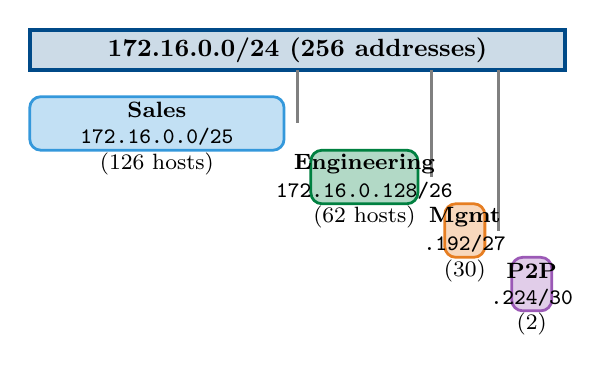
\begin{tikzpicture}[scale=0.85]
                    % Main network bar at top
                    \draw[fill=rctcblue!20, draw=rctcblue, line width=1.5pt] 
                        (0,4) rectangle (8,4.6);
                    \node[font=\small\bfseries] at (4,4.3) {172.16.0.0/24 (256 addresses)};
                    
                    % Dividing lines
                    \draw[line width=1pt, gray] (4,4) -- (4,3.2);
                    \draw[line width=1pt, gray] (6,4) -- (6,2.4);
                    \draw[line width=1pt, gray] (7,4) -- (7,1.6);
                    
                    % Sales subnet (largest)
                    \draw[fill=ipblue!30, draw=ipblue, line width=1pt, rounded corners] 
                        (0,2.8) rectangle (3.8,3.6);
                    \node[font=\footnotesize\bfseries] at (1.9,3.4) {Sales};
                    \node[font=\footnotesize\ttfamily] at (1.9,3.0) {172.16.0.0/25};
                    \node[font=\footnotesize] at (1.9,2.6) {(126 hosts)};
                    
                    % Engineering subnet
                    \draw[fill=networkgreen!30, draw=networkgreen, line width=1pt, rounded corners] 
                        (4.2,2) rectangle (5.8,2.8);
                    \node[font=\footnotesize\bfseries] at (5,2.6) {Engineering};
                    \node[font=\footnotesize\ttfamily] at (5,2.2) {172.16.0.128/26};
                    \node[font=\footnotesize] at (5,1.8) {(62 hosts)};
                    
                    % Management subnet
                    \draw[fill=aborange!30, draw=aborange, line width=1pt, rounded corners] 
                        (6.2,1.2) rectangle (6.8,2);
                    \node[font=\footnotesize\bfseries] at (6.5,1.8) {Mgmt};
                    \node[font=\footnotesize\ttfamily] at (6.5,1.4) {.192/27};
                    \node[font=\footnotesize] at (6.5,1) {(30)};
                    
                    % Point-to-point
                    \draw[fill=ippurple!30, draw=ippurple, line width=1pt, rounded corners] 
                        (7.2,0.4) rectangle (7.8,1.2);
                    \node[font=\footnotesize\bfseries] at (7.5,1) {P2P};
                    \node[font=\footnotesize\ttfamily] at (7.5,0.6) {.224/30};
                    \node[font=\footnotesize] at (7.5,0.2) {(2)};
                \end{tikzpicture}
            \end{center}

\articleonly{
\par\small\emph{This hierarchical VLSM diagram shows efficient subnet allocation from the 172.16.0.0/24 network using Variable Length Subnet Masking. Four subnets of different sizes are represented as colored boxes scaled proportionally to their capacity: Sales (blue, /25 with 126 hosts), Engineering (green, /26 with 62 hosts), Management (orange, /27 with 30 hosts), and a point-to-point link (purple, /30 with just 2 usable addresses). This demonstrates how VLSM allows precise address allocation matching actual requirements—using 220 total addresses for 177 hosts instead of wasting a full /23 (512 addresses) that fixed-length subnetting would require.}\par
}
            
            \vspace{0.2em}
            \begin{exampleblock}{Result}
                \small
                Used 220 addresses for 177 hosts. \\
                Without VLSM: would need 512+ addresses!
            \end{exampleblock}
        \end{column}
    \end{columns}
\end{frame}

% =============================================================================
% SLIDE 25: Case Study - Springfield Elementary Network Design
% =============================================================================
\begin{frame}{Case Study: Springfield Elementary Network Design}
    \begin{casestudy}{Springfield Elementary Network Design}
        Principal Skinner needs to design the school network with three segments. The district IT department has assigned him \texttt{172.16.50.0/24} (256 addresses).
        
        \vspace{0.5em}
        \begin{center}
            \scriptsize
            \begin{tabular}{l c l}
                \textbf{Segment} & \textbf{Devices Needed} & \textbf{Description} \\
                \midrule
                Computer Lab & 28 & Student workstations \\
                Admin Office & 12 & Staff computers, printers \\
                Teacher's Lounge & 6 & Laptops, smart TV \\
            \end{tabular}
        \end{center}
        
        Skinner wants to use VLSM to efficiently allocate addresses without waste.
    \end{casestudy}
    
    \begin{block}{Review Questions}
        \begin{enumerate}
            \small
            \item What is the smallest subnet size that can fit 28 hosts?
            \item List appropriate subnet assignments for each segment.
            \item How many addresses will be ``wasted'' (unused or reserved)?
        \end{enumerate}
    \end{block}
\end{frame}

% =============================================================================
% SLIDE 26: Case Study Solution - Springfield Elementary Network Design
% =============================================================================
\begin{frame}{Case Study Solution: Springfield Elementary Network Design}
    \begin{casesolution}{Springfield Elementary Network Design}
        \begin{enumerate}
            \item 28 hosts needs at least 30 usable addresses $\rightarrow$ \textbf{/27} (32 addresses, 30 usable).
            \item Subnet assignments (largest first):
        \end{enumerate}
    \end{casesolution}
    
    \vspace{0.2em}
    \begin{center}
        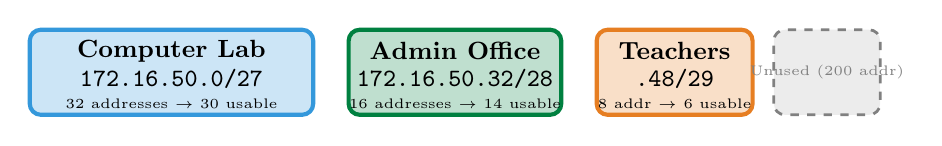
\begin{tikzpicture}[scale=0.9]
            % Computer Lab
            \draw[fill=ipblue!25, draw=ipblue, line width=1.5pt, rounded corners]
                (0,0) rectangle (4,1.2);
            \node[font=\small\bfseries] at (2,0.9) {Computer Lab};
            \node[font=\small\ttfamily] at (2,0.5) {172.16.50.0/27};
            \node[font=\tiny] at (2,0.15) {32 addresses $\rightarrow$ 30 usable};
            
            % Admin Office
            \draw[fill=networkgreen!25, draw=networkgreen, line width=1.5pt, rounded corners]
                (4.5,0) rectangle (7.5,1.2);
            \node[font=\small\bfseries] at (6,0.9) {Admin Office};
            \node[font=\small\ttfamily] at (6,0.5) {172.16.50.32/28};
            \node[font=\tiny] at (6,0.15) {16 addresses $\rightarrow$ 14 usable};
            
            % Teacher's Lounge
            \draw[fill=aborange!25, draw=aborange, line width=1.5pt, rounded corners]
                (8,0) rectangle (10.2,1.2);
            \node[font=\small\bfseries] at (9.1,0.9) {Teachers};
            \node[font=\small\ttfamily] at (9.1,0.5) {.48/29};
            \node[font=\tiny] at (9.1,0.15) {8 addr $\rightarrow$ 6 usable};
            
            % Unused space indicator
            \draw[fill=gray!15, draw=gray, line width=1pt, dashed, rounded corners]
                (10.5,0) rectangle (12,1.2);
            \node[font=\tiny, gray] at (11.25,0.6) {Unused (200 addr)};
        \end{tikzpicture}
    \end{center}

\articleonly{
\par\small\emph{This practical VLSM example shows address allocation for Springfield Elementary School's network using base 172.16.50.0. Three subnets are allocated with right-sized masks: Computer Lab (blue, /27 providing 30 usable addresses for 28 student PCs), Admin Office (green, /28 yielding 14 usable addresses for 12 staff devices), and Teachers' Lounge (orange, /29 giving 6 usable addresses for 6 faculty devices). A gray dashed box represents approximately 200 unused addresses remaining for future growth. The address accounting block shows that only 56 addresses were allocated to serve 46 devices with just 6 reserved for network/broadcast addresses and 4 "wasted" as appropriate headroom, demonstrating efficient address utilization through VLSM.}\par
}

    \vspace{0.2em}
    \begin{columns}[T]
        \begin{column}{0.48\textwidth}
            \begin{block}{Address Accounting}
                \small
                Used: $32 + 16 + 8 = 56$ addresses \\
                For: $28 + 12 + 6 = 46$ devices \\
                Reserved (net/bcast): 6 addresses \\
                ``Wasted'': 4 addresses (headroom)
            \end{block}
        \end{column}
        \begin{column}{0.48\textwidth}
            \begin{exampleblock}{Key Lesson}
                \small
                VLSM lets you right-size subnets. Always assign \textbf{largest first}, then work down. Leave room for growth!
            \end{exampleblock}
        \end{column}
    \end{columns}
\end{frame}

% =============================================================================
% SLIDE 27: ipconfig (Windows)
% =============================================================================
\section{IP Configuration and Diagnostics}
\subsection{Host Tools and Connectivity Testing}

\articleonly{
This section reviews host-side IP tools and a systematic approach to connectivity testing and troubleshooting.
}

\begin{frame}{ipconfig (Windows)}
    \begin{columns}[T]
        \begin{column}{0.45\textwidth}
            \begin{block}{Common Commands}
                \small
                \texttt{\textbf{ipconfig}} \\
                Shows IP, mask, gateway
                
                \vspace{0.3em}
                \texttt{\textbf{ipconfig /all}} \\
                Adds MAC, DHCP server, DNS
                
                \vspace{0.3em}
                \texttt{\textbf{ipconfig /release}} \\
                Release current DHCP lease
                
                \vspace{0.3em}
                \texttt{\textbf{ipconfig /renew}} \\
                Request new DHCP lease
                
                \vspace{0.3em}
                \texttt{\textbf{ipconfig /flushdns}} \\
                Clear the DNS cache
            \end{block}
        \end{column}
        \begin{column}{0.52\textwidth}
            \begin{block}{Sample Output: ipconfig /all}
                \ttfamily\tiny
                Ethernet adapter Local Area Connection:
                
                \vspace{0.2em}
                \begin{tabular}{@{}l l@{}}
                   Description & Intel Ethernet \\
                   Physical Address & \textcolor{networkgreen}{00-1A-2B-3C-4D-5E} \\
                   DHCP Enabled & Yes \\
                   IPv4 Address & \textcolor{ipblue}{192.168.1.100} \\
                   Subnet Mask & \textcolor{ipblue}{255.255.255.0} \\
                   Default Gateway & \textcolor{ipblue}{192.168.1.1} \\
                   DHCP Server & 192.168.1.1 \\
                   DNS Servers & 8.8.8.8 \\
                \end{tabular}
            \end{block}
            
            \vspace{0.2em}
            \begin{alertblock}{Troubleshooting Tip}
                \small
                See \texttt{169.254.x.x}? DHCP failed! \\
                See \texttt{0.0.0.0}? No IP assigned at all.
            \end{alertblock}
        \end{column}
    \end{columns}
\end{frame}

% =============================================================================
% SLIDE 28: ifconfig and ip (Linux)
% =============================================================================
\begin{frame}{ifconfig and ip (Linux)}
    \begin{columns}[T]
        \begin{column}{0.48\textwidth}
            \begin{block}{Legacy: ifconfig}
                \small
                \texttt{\textbf{ifconfig}} \\
                Show all interface configuration
                
                \vspace{0.3em}
                \texttt{\textbf{ifconfig eth0}} \\
                Show specific interface
                
                \vspace{0.3em}
                \texttt{\textbf{ifconfig eth0 down}} \\
                Disable an interface
                
                \vspace{0.3em}
                \texttt{\textbf{ifconfig eth0 up}} \\
                Enable an interface
            \end{block}
            
            \vspace{0.2em}
            \begin{alertblock}{Note}
                \small
                \texttt{ifconfig} is deprecated on many modern Linux distributions. Use \texttt{ip} instead!
            \end{alertblock}
        \end{column}
        \begin{column}{0.48\textwidth}
            \begin{block}{Modern: ip command}
                \small
                \texttt{\textbf{ip addr}} (or \texttt{ip a}) \\
                Show IP addresses
                
                \vspace{0.3em}
                \texttt{\textbf{ip link}} \\
                Show interface status (up/down)
                
                \vspace{0.3em}
                \texttt{\textbf{ip route}} \\
                Show routing table and gateway
                
                \vspace{0.3em}
                \texttt{\textbf{ip neigh}} \\
                Show ARP cache (neighbors)
            \end{block}
            
            \vspace{0.2em}
            \begin{exampleblock}{Sample: ip addr}
                \ttfamily\tiny
                2: eth0: <UP,BROADCAST> \\
                \quad inet \textcolor{ipblue}{192.168.1.50/24} \\
                \quad link/ether \textcolor{networkgreen}{00:1a:2b:3c:4d:5e}
            \end{exampleblock}
        \end{column}
    \end{columns}
\end{frame}

% =============================================================================
% SLIDE 29: The arp Command
% =============================================================================
\begin{frame}{The arp Command}
    \begin{columns}[T]
        \begin{column}{0.48\textwidth}
            \begin{block}{Common Commands}
                \small
                \texttt{\textbf{arp -a}} \\
                Display entire ARP cache
                
                \vspace{0.3em}
                \texttt{\textbf{arp -a 192.168.1.1}} \\
                Display entry for specific IP
                
                \vspace{0.3em}
                \texttt{\textbf{arp -d 192.168.1.1}} \\
                Delete an entry from cache
                
                \vspace{0.3em}
                \texttt{\textbf{arp -s 192.168.1.1 00-1a-2b-3c-4d-5e}} \\
                Add a static entry manually
            \end{block}
            
            \vspace{0.2em}
            \begin{alertblock}{When to Use}
                \small
                \begin{itemize}
                    \item Verify local connectivity
                    \item Troubleshoot duplicate IPs
                    \item Check for ARP poisoning
                    \item Force re-resolution of MAC
                \end{itemize}
            \end{alertblock}
        \end{column}
        \begin{column}{0.48\textwidth}
            \begin{block}{Sample Output: arp -a}
                \ttfamily\tiny
                Interface: 192.168.1.100 \\
                \vspace{0.2em}
                \begin{tabular}{@{}l l l@{}}
                    \textbf{Internet Addr} & \textbf{Physical Addr} & \textbf{Type} \\
                    192.168.1.1 & 00-1a-2b-3c-4d-01 & dynamic \\
                    192.168.1.25 & 00-1a-2b-3c-4d-25 & dynamic \\
                    192.168.1.50 & 00-1a-2b-3c-4d-50 & dynamic \\
                    192.168.1.254 & 00-1a-2b-3c-4d-fe & static \\
                \end{tabular}
            \end{block}
            
            \vspace{0.3em}
            \begin{exampleblock}{Dynamic vs Static}
                \small
                \textbf{Dynamic}: Learned via ARP, expires after timeout
                
                \vspace{0.2em}
                \textbf{Static}: Manually configured, never expires
            \end{exampleblock}
        \end{column}
    \end{columns}
\end{frame}

% =============================================================================
% SLIDE 30: ping - The Essential Test
% =============================================================================
\begin{frame}{ping: The Essential Connectivity Test}
    \begin{columns}[T]
        \begin{column}{0.48\textwidth}
            \begin{itemize}
                \item \texttt{ping} tests reachability using \keyterm{ICMP} echo request/reply.
                \item Measures \keyterm{round-trip time (RTT)} in milliseconds.
                \item \keyterm{TTL} in response indicates hops traveled.
                \item Works on Windows, Linux, Mac.
            \end{itemize}
            
            \vspace{0.3em}
            \begin{block}{Common Options}
                \small
                \texttt{\textbf{ping 192.168.1.1}} \\
                Basic connectivity test
                
                \vspace{0.2em}
                \texttt{\textbf{ping -t 192.168.1.1}} \\
                Continuous ping -- Windows
                
                \vspace{0.2em}
                \texttt{\textbf{ping -c 5 192.168.1.1}} \\
                Send 5 pings -- Linux/Mac
            \end{block}
        \end{column}
        \begin{column}{0.48\textwidth}
            \begin{block}{Sample Output}
                \ttfamily\tiny
                Pinging 192.168.1.1 with 32 bytes of data:
                
                \vspace{0.2em}
                Reply from 192.168.1.1: bytes=32 \textcolor{networkgreen}{time=2ms} \textcolor{ipblue}{TTL=64} \\
                Reply from 192.168.1.1: bytes=32 \textcolor{networkgreen}{time=1ms} \textcolor{ipblue}{TTL=64} \\
                Reply from 192.168.1.1: bytes=32 \textcolor{networkgreen}{time=1ms} \textcolor{ipblue}{TTL=64} \\
                Reply from 192.168.1.1: bytes=32 \textcolor{networkgreen}{time=2ms} \textcolor{ipblue}{TTL=64}
            \end{block}
            
            \vspace{0.3em}
            \begin{alertblock}{Common Results}
                \small
                \textbf{Reply} -- Success! Host is reachable
                
                \vspace{0.1em}
                \textbf{Request timed out} -- No response received
                
                \vspace{0.1em}
                \textbf{Destination unreachable} -- Routing problem
            \end{alertblock}
        \end{column}
    \end{columns}
\end{frame}

% =============================================================================
% SLIDE 31: Ping Troubleshooting Methodology
% =============================================================================
\begin{frame}{Ping Troubleshooting Methodology}
    \begin{center}
        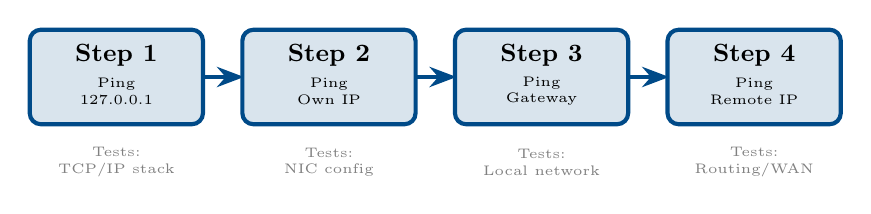
\begin{tikzpicture}[scale=0.9]
            % Step boxes
            \node[draw=rctcblue, fill=rctcblue!15, line width=1.5pt, rounded corners,
                  minimum width=2.2cm, minimum height=1.2cm] (s1) at (0,0) {};
            \node[font=\small\bfseries] at (0,0.3) {Step 1};
            \node[font=\tiny, align=center] at (0,-0.2) {Ping\\127.0.0.1};
            
            \node[draw=rctcblue, fill=rctcblue!15, line width=1.5pt, rounded corners,
                  minimum width=2.2cm, minimum height=1.2cm] (s2) at (3,0) {};
            \node[font=\small\bfseries] at (3,0.3) {Step 2};
            \node[font=\tiny, align=center] at (3,-0.2) {Ping\\Own IP};
            
            \node[draw=rctcblue, fill=rctcblue!15, line width=1.5pt, rounded corners,
                  minimum width=2.2cm, minimum height=1.2cm] (s3) at (6,0) {};
            \node[font=\small\bfseries] at (6,0.3) {Step 3};
            \node[font=\tiny, align=center] at (6,-0.2) {Ping\\Gateway};
            
            \node[draw=rctcblue, fill=rctcblue!15, line width=1.5pt, rounded corners,
                  minimum width=2.2cm, minimum height=1.2cm] (s4) at (9,0) {};
            \node[font=\small\bfseries] at (9,0.3) {Step 4};
            \node[font=\tiny, align=center] at (9,-0.2) {Ping\\Remote IP};
            
            % Arrows
            \draw[-{Stealth}, line width=1.5pt, rctcblue] (1.2,0) -- (1.8,0);
            \draw[-{Stealth}, line width=1.5pt, rctcblue] (4.2,0) -- (4.8,0);
            \draw[-{Stealth}, line width=1.5pt, rctcblue] (7.2,0) -- (7.8,0);
            
            % What it tests - below each box
            \node[font=\tiny, align=center, gray] at (0,-1.2) {Tests:\\TCP/IP stack};
            \node[font=\tiny, align=center, gray] at (3,-1.2) {Tests:\\NIC config};
            \node[font=\tiny, align=center, gray] at (6,-1.2) {Tests:\\Local network};
            \node[font=\tiny, align=center, gray] at (9,-1.2) {Tests:\\Routing/WAN};
        \end{tikzpicture}
    \end{center}
    
    \vspace{0.5em}
    \begin{columns}[T]
        \begin{column}{0.48\textwidth}
            \begin{block}{If Step 1 Fails}
                \small
                TCP/IP stack is broken. Reinstall network drivers or reset TCP/IP stack.
            \end{block}
            
            \vspace{0.2em}
            \begin{block}{If Step 2 Fails}
                \small
                NIC is not configured properly. Check IP settings, cable, NIC driver.
            \end{block}
        \end{column}
        \begin{column}{0.48\textwidth}
            \begin{block}{If Step 3 Fails}
                \small
                Local network issue. Check cable, switch port, gateway address, ARP table.
            \end{block}
            
            \vspace{0.2em}
            \begin{block}{If Step 4 Fails}
                \small
                Routing or remote issue. Check gateway config, ISP connection, firewall.
            \end{block}
        \end{column}
    \end{columns}
\end{frame}

% =============================================================================
% SLIDE 32: Why IPv6?
% =============================================================================
\section{IPv6 Fundamentals}
\subsection{Addressing, Types, and Transition}

\articleonly{
The final section introduces IPv6 structure, address types, and migration approaches from IPv4 environments.
}

\begin{frame}{Why IPv6? The Problem with IPv4}
    \begin{columns}[T]
        \begin{column}{0.48\textwidth}
            \begin{itemize}
                \item IPv4 has only about \textbf{4.3 billion} addresses.
                \item Already exhausted! IANA ran out in 2011.
                \item Workarounds like NAT and CIDR helped, but add complexity.
                \item \keyterm{IPv6} provides a permanent solution.
            \end{itemize}
            
            \vspace{0.3em}
            \begin{alertblock}{IPv6 Address Space}
                $2^{128}$ = 340 undecillion addresses
                
                \vspace{0.2em}
                That's 340,282,366,920,938,463,463,\\374,607,431,768,211,456 addresses!
            \end{alertblock}
        \end{column}
        \begin{column}{0.48\textwidth}
            \begin{block}{IPv6 Benefits}
                \begin{itemize}
                    \item Virtually unlimited addresses
                    \item Simpler header format
                    \item Built-in IPsec support
                    \item No need for NAT
                    \item Auto-configuration -- SLAAC
                    \item Better multicast support
                \end{itemize}
            \end{block}
            
            \vspace{0.3em}
            \begin{exampleblock}{Perspective}
                \small
                IPv6 could assign a unique address to every atom on Earth's surface... and still have addresses left over!
            \end{exampleblock}
        \end{column}
    \end{columns}
\end{frame}

% =============================================================================
% SLIDE 33: IPv6 Address Format
% =============================================================================
\begin{frame}{IPv6 Address Format}
    \begin{columns}[T]
        \begin{column}{0.45\textwidth}
            \begin{itemize}
                \item \textbf{128 bits} long -- 4x longer than IPv4.
                \item Written as 8 groups of 4 hex digits.
                \item Groups separated by colons.
                \item Letters can be uppercase or lowercase.
            \end{itemize}
            
            \vspace{0.3em}
            \begin{block}{Full Format}
                \ttfamily\small
                2001:0db8:85a3:0000:\\0000:8a2e:0370:7334
            \end{block}
        \end{column}
        \begin{column}{0.52\textwidth}
            \begin{block}{Simplification Rules}
                \small
                \textbf{Rule 1}: Drop leading zeros in each group
                
                \vspace{0.2em}
                \ttfamily\footnotesize
                2001:\textcolor{alertred}{0}db8:85a3:\textcolor{alertred}{000}0:\textcolor{alertred}{000}0:8a2e:\textcolor{alertred}{0}370:7334
                
                \vspace{0.1em}
                $\downarrow$
                
                \vspace{0.1em}
                2001:db8:85a3:0:0:8a2e:370:7334
                
                \vspace{0.4em}
                \normalfont
                \textbf{Rule 2}: Replace ONE set of consecutive zero groups with ::
                
                \vspace{0.2em}
                \ttfamily\footnotesize
                2001:db8:85a3:\textcolor{alertred}{0:0}:8a2e:370:7334
                
                \vspace{0.1em}
                $\downarrow$
                
                \vspace{0.1em}
                2001:db8:85a3\textcolor{networkgreen}{::}8a2e:370:7334
            \end{block}
        \end{column}
    \end{columns}
    
    \vspace{0.3em}
    \begin{alertblock}{Important: Use :: Only Once!}
        You can only use :: once per address. Using it twice would make the address ambiguous -- you wouldn't know how many zero groups each :: represents.
    \end{alertblock}
\end{frame}

% =============================================================================
% SLIDE 34: IPv6 Network Prefixes and Address Types
% =============================================================================
\begin{frame}{IPv6 Network Prefixes and Address Types}
    \begin{columns}[T]
        \begin{column}{0.45\textwidth}
            \begin{itemize}
                \item IPv6 uses \keyterm{prefix length} instead of subnet mask.
                \item Written with slash notation: \texttt{/64}
                \item Standard subnet prefix: \textbf{/64}
                \item First 64 bits = network, last 64 bits = interface ID.
            \end{itemize}
            
            \vspace{0.3em}
            \begin{center}
                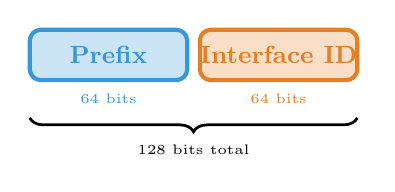
\begin{tikzpicture}[scale=0.8]
                    % Network prefix box
                    \draw[fill=ipblue!25, draw=ipblue, line width=1.5pt, rounded corners]
                        (0,0) rectangle (2.5,0.8);
                    \node[font=\small\bfseries, ipblue] at (1.25,0.4) {Prefix};
                    
                    % Interface ID box
                    \draw[fill=aborange!25, draw=aborange, line width=1.5pt, rounded corners]
                        (2.7,0) rectangle (5.2,0.8);
                    \node[font=\small\bfseries, aborange] at (3.95,0.4) {Interface ID};
                    
                    % Bit labels below
                    \node[font=\tiny, ipblue] at (1.25,-0.3) {64 bits};
                    \node[font=\tiny, aborange] at (3.95,-0.3) {64 bits};
                    
                    % Total label
                    \draw[decorate, decoration={brace, amplitude=5pt, mirror}, line width=1pt]
                        (0,-0.6) -- (5.2,-0.6);
                    \node[font=\tiny] at (2.6,-1.1) {128 bits total};
                \end{tikzpicture}
            \end{center}
        \end{column}
        \begin{column}{0.52\textwidth}
            \begin{block}{Common IPv6 Address Types}
                \small
                \begin{tabular}{l l}
                    \toprule
                    \textbf{Type} & \textbf{Prefix} \\
                    \midrule
                    Global Unicast & 2000::/3 \\
                    Link-Local & fe80::/10 \\
                    Unique Local & fc00::/7 \\
                    Multicast & ff00::/8 \\
                    Loopback & ::1/128 \\
                    Unspecified & ::/128 \\
                    \bottomrule
                \end{tabular}
            \end{block}
            
            \vspace{0.2em}
            \begin{exampleblock}{Example Address}
                \ttfamily\small
                2001:db8:1234:5678::1/64
                
                \vspace{0.2em}
                \normalfont\small
                Prefix: 2001:db8:1234:5678 \\
                Interface ID: ::1
            \end{exampleblock}
        \end{column}
    \end{columns}
\end{frame}

% =============================================================================
% SLIDE 35: IPv6 Address Types Explained
% =============================================================================
\begin{frame}[t,shrink=12]{IPv6 Address Types Explained}
    \begin{columns}[T]
        \begin{column}{0.48\textwidth}
            \begin{block}{Global Unicast -- GUA}
                \small
                \begin{itemize}
                    \item Public, routable addresses
                    \item Equivalent to IPv4 public IPs
                    \item Start with 2 or 3
                    \item Assigned by ISPs
                \end{itemize}
            \end{block}
            
            \vspace{0.2em}
            \begin{block}{Link-Local -- fe80::}
                \small
                \begin{itemize}
                    \item Auto-configured on every interface
                    \item Only valid on local segment
                    \item NOT routable
                    \item Used for neighbor discovery
                \end{itemize}
            \end{block}
            
            \vspace{0.2em}
            \begin{alertblock}{Always Present}
                \small
                Every IPv6 interface has a link-local address, even without DHCP or manual config!
            \end{alertblock}
        \end{column}
        \begin{column}{0.48\textwidth}
            \begin{block}{Unique Local -- fc00::/7}
                \small
                \begin{itemize}
                    \item Private addresses
                    \item Like IPv4 10.x.x.x or 192.168.x.x
                    \item NOT routable on internet
                    \item For internal use only
                \end{itemize}
            \end{block}
            
            \vspace{0.2em}
            \begin{block}{Multicast -- ff00::/8}
                \small
                \begin{itemize}
                    \item One-to-many communication
                    \item Replaces IPv4 broadcast
                    \item ff02::1 = all nodes
                    \item ff02::2 = all routers
                \end{itemize}
            \end{block}
            
            \vspace{0.2em}
            \begin{exampleblock}{Loopback}
                \small
                \texttt{::1} is the IPv6 loopback -- equivalent to IPv4's 127.0.0.1
            \end{exampleblock}
        \end{column}
    \end{columns}
\end{frame}

% =============================================================================
% SLIDE 36: IPv4 to IPv6 Transition
% =============================================================================
\begin{frame}[t,shrink=20]{IPv4 to IPv6 Transition}
    \begin{columns}[T]
        \begin{column}{0.48\textwidth}
            \begin{block}{Dual Stack}
                \begin{itemize}
                    \small
                    \item Run IPv4 AND IPv6 simultaneously
                    \item Most common transition method
                    \item Devices have both addresses
                    \item Gradual migration over time
                \end{itemize}
                
                \centering
                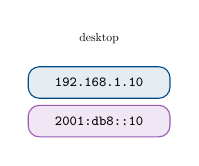
\begin{tikzpicture}[scale=0.7]
                    \node[pc] (pc) at (0,0) {\iconpc[0.5cm]};
                    \node[ipbox, font=\tiny\ttfamily, minimum width=1.8cm] at (0,-0.8) {192.168.1.10};
                    \node[ipbox, font=\tiny\ttfamily, minimum width=1.8cm, fill=ippurple!15, draw=ippurple] at (0,-1.5) {2001:db8::10};
                \end{tikzpicture}
            \end{block}
        \end{column}
        \begin{column}{0.48\textwidth}
            \begin{block}{Tunneling}
                \begin{itemize}
                    \scriptsize
                    \item Encapsulate IPv6 inside IPv4
                    \item Cross IPv4-only networks
                    \item Types: 6to4, Teredo, ISATAP
                    \item Adds overhead
                \end{itemize}
            \end{block}
            
            \vspace{0.2em}
            \begin{block}{Translation -- NAT64}
                \begin{itemize}
                    \scriptsize
                    \item Convert between protocols
                    \item IPv6-only hosts reach IPv4 servers
                    \item More complex to manage
                    \item Last resort option
                \end{itemize}
            \end{block}
        \end{column}
    \end{columns}
    
    \begin{exampleblock}{Recommendation}
        \scriptsize
        \textbf{Dual stack} is the preferred transition method. Run both protocols until IPv4 can be safely retired. Most modern operating systems support dual stack by default.
    \end{exampleblock}
\end{frame}

% =============================================================================
% SLIDE 37: Module 4.0 Summary
% =============================================================================
\section*{Module Summary}

\begin{frame}[t,allowframebreaks]{Module 4.0 Summary}
    \small
    \textbf{Key Concepts:}
    \begin{itemize}
        \item \keyterm{IP (Layer 3)} provides end-to-end addressing; \keyterm{MAC (Layer 2)} provides local delivery. \keyterm{ARP} resolves IP to MAC.
        \item \keyterm{IPv4 addresses}: 32-bit dotted decimal (e.g., 192.168.1.100). \keyterm{Subnet mask} divides network and host portions.
        \item \keyterm{CIDR notation} (e.g., /24) replaced classful addressing. Usable hosts = $2^n - 2$ (subtract network and broadcast addresses).
        \item \keyterm{VLSM} (Variable Length Subnet Masking) allows subnets of different sizes for efficient IP allocation.
        \item \keyterm{Private IP ranges}: 10.0.0.0/8, 172.16.0.0/12, 192.168.0.0/16 (RFC 1918). Use \keyterm{NAT} for internet access.
        \item Address types: \keyterm{Unicast} (one-to-one), \keyterm{Broadcast} (one-to-all on subnet), \keyterm{Multicast} (one-to-group), \keyterm{Anycast} (one-to-nearest).
        \item \keyterm{Default gateway} must be on the same subnet as the host. \keyterm{TTL} (Time to Live) prevents routing loops.
    \end{itemize}
    \framebreak
    
    \vspace{0.3em}
    \textbf{Troubleshooting \& IPv6:}
    \begin{itemize}
        \item Tools: \keyterm{ipconfig/ifconfig} (view config), \keyterm{ping} (test connectivity), \keyterm{arp} (view MAC mappings), \keyterm{traceroute} (show path).
        \item Methodology: Ping loopback (127.0.0.1) $\rightarrow$ local gateway $\rightarrow$ remote host to isolate problems.
        \item \keyterm{169.254.x.x} = APIPA (DHCP failure). Empty ARP table indicates Layer 1/2 problem.
        \item \keyterm{IPv6}: 128-bit addresses in hex notation (e.g., 2001:db8::1). Use :: to compress zeros.
        \item IPv6 types: \keyterm{Link-local} (fe80::/10, auto-configured), \keyterm{Global unicast} (2000::/3), \keyterm{Unique local} (fc00::/7).
        \item \keyterm{Dual stack}: Run IPv4 and IPv6 simultaneously during transition period.
    \end{itemize}
\end{frame}

\articleonly{
\subsection*{Conclusion}
This module covered IPv4 and IPv6 addressing, subnetting with CIDR and VLSM, address resolution with ARP, and troubleshooting tools. You learned to calculate subnet masks, plan IP address schemes, and diagnose connectivity problems systematically. In the next module, we'll explore routing protocols and how packets travel between networks.
}


\end{document}


